%%%%%%%%%%%%%%%%%%%%%%%%%%%%%%%%%%%%%%%%%%%%%%%%%%%%%%%%%%%%%%%%%%%%%%%%%%%%%%%%
%%%%%%%%%%%%%%%%%%   Vorlage für eine Abschlussarbeit   %%%%%%%%%%%%%%%%%%%%%%%%
%%%%%%%%%%%%%%%%%%%%%%%%%%%%%%%%%%%%%%%%%%%%%%%%%%%%%%%%%%%%%%%%%%%%%%%%%%%%%%%%

% Erstellt von Maximilian Nöthe, <maximilian.noethe@tu-dortmund.de>
% ausgelegt für lualatex und Biblatex mit biber

% Kompilieren mit
% lualatex dateiname.tex
% biber dateiname.bcf
% lualatex dateiname.tex
% lualatex dateiname.tex
% oder einfach mit:
% make

\documentclass[
  tucolor,
  BCOR=12mm,     % 12mm binding corrections, adjust to fit your binding
  parskip=half,  % new paragraphs start with half line vertical space
  open=any,      % chapters start on both odd and even pages
  cleardoublepage=plain,  % no header/footer on blank pages
]{tudothesis}

% \usepackage{geometry}
% \geometry{a4paper, margin=2.5cm, top=3.5cm}
% \usepackage[onehalfspacing]{setspace}

% Warning, if another latex run is needed
\usepackage[aux]{rerunfilecheck}

% just list chapters and sections in the toc, not subsections or smaller
\setcounter{tocdepth}{1}

%------------------------------------------------------------------------------
%------------------------------ Sprache und Schrift: --------------------------
%------------------------------------------------------------------------------
\usepackage{fontspec}
\defaultfontfeatures{Ligatures=TeX}  % -- becomes en-dash etc.

% german language
\usepackage{polyglossia}
\setdefaultlanguage{english}

% for german parts if needed
\setotherlanguages{german}

% intelligent quotation marks, language and nesting sensitive
\usepackage[autostyle]{csquotes}

% microtypographical features, makes the text look nicer on the small scale
\usepackage{microtype}

%------------------------------------------------------------------------------
%------------------------ Für die Matheumgebung--------------------------------
%------------------------------------------------------------------------------

\usepackage{amsmath}
\usepackage{amssymb}
\usepackage{mathtools}

% Enable Unicode-Math and follow the ISO-Standards for typesetting math
\usepackage[
  math-style=ISO,
  bold-style=ISO,
  sans-style=italic,
  nabla=upright,
  partial=upright,
]{unicode-math}
\setmathfont{Latin Modern Math}

% nice, small fracs for the text with \sfrac{}{}
\usepackage{xfrac}


%------------------------------------------------------------------------------
%---------------------------- Numbers and Units -------------------------------
%------------------------------------------------------------------------------

\usepackage[
  locale=DE,
  separate-uncertainty=true,
  per-mode=symbol-or-fraction,
]{siunitx}
\sisetup{math-micro=\text{µ},text-micro=µ,range-phrase=-}

%------------------------------------------------------------------------------
%-------------------------------- tables  -------------------------------------
%------------------------------------------------------------------------------

\usepackage{booktabs}       % stellt \toprule, \midrule, \bottomrule

%------------------------------------------------------------------------------
%-------------------------------- graphics -------------------------------------
%------------------------------------------------------------------------------

\usepackage{graphicx}
\usepackage{grffile}
\usepackage{subcaption}

% allow figures to be placed in the running text by default:
\usepackage{scrhack}
\usepackage{float}
\floatplacement{figure}{htbp}
\floatplacement{table}{htbp}

% keep figures and tables in the section
\usepackage[section, below]{placeins}


%------------------------------------------------------------------------------
%---------------------- customize list environments ---------------------------
%------------------------------------------------------------------------------

\usepackage{enumitem}

%------------------------------------------------------------------------------
%------------------------------ Bibliographie ---------------------------------
%------------------------------------------------------------------------------

\usepackage[
  backend=biber,   % use modern biber backend
  autolang=hyphen, % load hyphenation rules for if language of bibentry is not
                   % german, has to be loaded with \setotherlanguages
                   % in the references.bib use langid={en} for english sources
]{biblatex}
\addbibresource{references.bib}  % die Bibliographie einbinden
\DefineBibliographyStrings{german}{andothers = {{et\,al\adddot}}}

\usepackage[labelformat=simple]{subcaption}
\renewcommand\thesubfigure{(\alph{subfigure})}

%------------------------------------------------------------------------------
%------------------------------ Sonstiges: ------------------------------------
%------------------------------------------------------------------------------

\usepackage[pdfusetitle,unicode,linkbordercolor=tugreen]{hyperref}
\usepackage{bookmark}
\usepackage[shortcuts]{extdash}
\usepackage{blindtext}
\usepackage{multicol}

%------------------------------------------------------------------------------
%------------------------------    TIKZ:   ------------------------------------
%------------------------------------------------------------------------------
\usepackage{tikz}
\usetikzlibrary{shapes.geometric, arrows}
\tikzstyle{edge from parent}=[tugreen,thick,draw]
\tikzstyle{feature} = [rectangle, minimum width=2cm, minimum height=1cm,text centered, draw=white, fill=tugreen]
\tikzstyle{class1} = [rectangle, minimum width=1cm, minimum height=0.75cm,text centered, draw=white, text=white, fill=black]
\tikzstyle{class2} = [rectangle, minimum width=1cm, minimum height=0.75cm,text centered, draw=black, fill=white]
\tikzstyle{pil} = [-, thick, color=tugreen, text=tugreen]

%------------------------------------------------------------------------------
%-------------------------    Angaben zur Arbeit   ----------------------------
%------------------------------------------------------------------------------

\author{Kevin Sedlaczek}
\title{Analysis of the Crab Nebula using Photon Stream data collected by FACT}
\date{\today}
\birthplace{Dortmund}
\chair{Lehrstuhl für Experimentelle Physik Vb}
\division{Fakultät Physik}
\thesisclass{Master of Science}
\submissiondate{31. Dezember 2018}
\firstcorrector{Prof.~Dr.~Dr.~Wolfgang Rħode}
\secondcorrector{Prof.~Dr.~Zweitkorrekteur}

% tu logo on top of the titlepage
\titlehead{
\includegraphics[height=1.5cm]{logos/tu-logo.pdf}}

\raggedbottom

\begin{document}
\frontmatter
% \input{content/hints.tex}
\maketitle

% Gutachterseite
\makecorrectorpage

% hier beginnt der Vorspann, nummeriert in römischen Zahlen
\chapter{Abstract}

This work is investigating the novel data format \textit{Photon Stream} by
analyzing physics data of the Crab Nebula. \textcolor{red}{Nicht vollständig}
\\
\\
In dieser Arbeit wird das neuartige Datenformat \textit{Photon Stream} im
Zusammhang einer Analyse des Krebsnebels untersucht.

\tableofcontents

\mainmatter
% Hier beginnt der Inhalt mit Seite 1 in arabischen Ziffern
\chapter{Introduction}
\nocite{biblatex, siunitx, Hunter:2007}%
%
\begin{aquote}{\textit{Albert Einstein}}
\textsc{One cannot help but be in awe when he contemplates the mysteries of eternity, of life, of the marvelous structure of reality.}
\end{aquote}
In physics, the search for a fundamental understanding of reality is ubiquitous. The understanding of the universe we live in and the rules of nature has
led mankind to look for the things beyond earth. To understand what these rules
are, on earth and in the universe, is the goal of astrophysics. The electromagnetic radiation reaching the earth from space has opened the window to learn
about the universe beyond our planet. The discovery of this extraterrestrial
radiation by Victor Hess during his balloon flights around \num{100} years ago in \num{1912}~\cite{Hess} marks the beginning of the observation of this radiation.
Today we know that the electromagnetic radiation spans a very large range of
frequencies and reaches up to the highest energies ever measured \cite{source}.
The different energy ranges of cosmic radiation caused the development of a
variety of different telescopes, specialized on certain frequency bands. On
ground, only visible light and radio waves from space can be observed directly,
due to the absorption of Earth's atmosphere. Therefore, large optical and radio
telescopes have been built to observe stars, galaxies and other objects from
Earth. Of course, the atmosphere still has an impact on the observations, so
there are optical telescopes in space as well, like the Hubble Space
Telescope~\cite{hubble}, observing infra-red to ultra-violett light. However,
some telescopes take advantage of the atmosphere's impact, by using it as a
giant detector volume. Among these telescopes are the Imaging Air Cherenkov
Telescopes (IACT), observing cosmic rays via their interaction products. This
work is based on the observations of such a telescope, described in
\autoref{ch:fact}. The development and advancement of new telescopes continues
today, as the currently constructed Cherenkov Telescope Array CTA~\cite{cta}
will yield unprecedented accuracy and sensitivity among IACTs.
Among the goals of astrophysics are not only the understanding of the
structures of the universe, but also the very elementary interactions of
particles within the sources of this radiation. The very first hints for the
existance and characteristics of dark matter~\cite{zwicky}, a supposed
elementary particle for instance originate from the field of astrophysics.
This work focuses on the rather technical aspect of a new data representation
and its implications for IACT analyses, by analyzing a data set of this new data
format for the first time.

\chapter{Imaging Air Cherenkov Astronomy}
\label{ch:iact}
%
\begin{figure}[H]
  \centering
  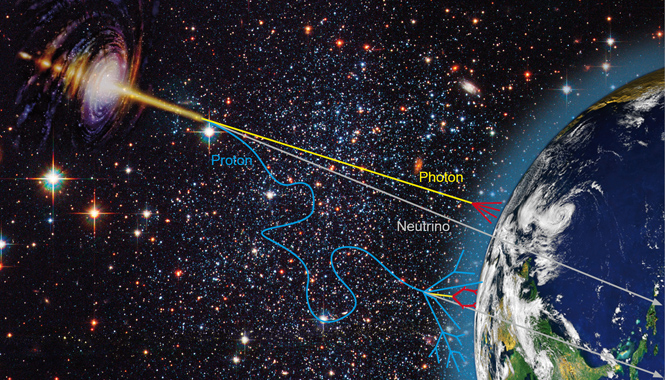
\includegraphics[width=0.95\textwidth]{Plots/cosmic_rays.jpg}
  \caption{Different constituents of the cosmic rays reaching earth \cite{cosmic-rays}. There are three different particle types of cosmic rays that can be used for astronomy. The uncharged and very light neutrinos (white) barely interact with anything on their way through the universe. Thus, they give strong hints on their origin, but are very hard to detect as well. The charged particles such as protons or ionized atoms (blue) are deflected by magnetic fields and therefore lose any direction information. Lastly, cosmic gamma-rays (yellow), massless uncharged photons, are emitted through various processes and from different sources such as active galctic nuclei. They are not deflected much and are the main signal for Cherenkov astronomy.}
  \label{fig:rays}
\end{figure}
%
The atmosphere of earth is continously penetrated by radiation from different
sources within our universe. This cosmic radiation is made up of different types
of particles, interacting with the atmosphere in various ways. There are
charged protons and the uncharged neutrinos and photons (gamma rays). Neutrinos
are uncharged, very light fermions, that interact very weakly and are not
detectable by optical telescopes at all. Protons make up the largest number of
particles reaching earths atmosphere. Due to their electric charge, they are
deflected by magnetic fields and therefore lose information on their origin on
the way to earth, making them unsuitable for Cherenkov astronomy.
%
\section{Cosmic Gamma-Rays}
%
Cosmic gamma-rays are photons with a very high energy, originating from bright
sources such as active galactic nuclei or nebulae. When such particles intersect
with earth's atmosphere, they create new particles moving faster than light
within that atmosphere due to their high energy. Particles moving at such
speeds through a medium cause, among the creation of other particles, the
emission of bluish photons, the Cherenkov-light.
Cherenkov-light is emitted by the medium directly from the moving particle
within a specific angle towards the direction of movement of that primary
particle.
%
\begin{equation}
    \cos(\vartheta) = \frac{1}{n\beta}
    \label{eq:angle_cherenkov}
\end{equation}
%
As \autoref{eq:angle_cherenkov} shows, this angle depends on the index of
refraction $n$ of the medium and the particle's velocity. Due to this emission
angle the light traverses the medium in a cone-shape, when being described from
earth's point of view. By the time it is reaching the ground it thus
illuminates an elliptical area of about $\SI{200}{\meter}$ diameter, depending
on the height of interaction and the primary particle's energy.
This already implicates that the light, although a secondary product of the
cosmic gamma-ray, can be used to reconstruct physical properties of
said gamma-ray. To do so, the flashes of the Cherenkov-light need to
be captured by cameras capable of filming very short time scales (about
$\SI{e-9}{\second}$).

\section{Imaging Air Cherenkov Telescopes}

Imaging Air Cherenkov Telescopes (IACTs) are using videos of this light, to
reconstruct properties of the incident cosmic radiation above
$\SI{100}{\giga\electronvolt}$, by analyzing the spatial geometry of the
measured pictures.

The three properties of interest for each event are:
%
\begin{description}[labelsep=1em]
  \item[source position]{the position of the source of the primary particle on the sky}
  \item[particle type]{the distinction between cosmic gamma rays and other particles like protons or secondary particles like muons}
  \item[particle energy]{the energy of the primary gamma-ray}
\end{description}
%
This means that the task is to resolve single incoming cosmic gamma rays and
reconstruct these properties. By doing so, the atmosphere is used as a very
wide spread detector. When trying to avoid any interactions of the incident
particles and measuring their properties directly in a specifically prepared
detector material, one eventuually has to leave earth's atmosphere. Such direct
measurements are carried out in earth's orbit, outside its atmosphere.
Detectors like the Fermi Large-Area-Telescope \cite{fermiLAT} (Fermi LAT) are satellites
carrying their own detectors for the necessary measurements. They consist of
interaction volumes taking over what the atmosphere does to intersecting cosmic
rays: particles like gamma rays interact with the material, creating new
particles by losing energy, which then continue to do so in particle cascades
until the energy has spread to a certain amount. This process is called
shower (or air-shower, depending on the medium of interaction). The
characteristics of these interactions and the produced particles strongly
depend on the properties of the incident particle, such as energy and particle
type. There are particles that mainly interact via the electromagnetic force.
Such showers are called electromagnetic showers. They are usually initiated by
photons or electrons and mainly consist of light, charged fermions like electrons or
muons and photons or light, charged bosons like pions. Showers initiated by
hadronic cosmic rays like protons show different kinds of interactions, also
resulting in different spatial topologies. The momentum perpendicular to the
primary particle's trajectory is bigger, giving the shower a wider spread of
secondary particles. This is the main characteristic to distinguish hadronic
showers, resembling the main background within the measurements (apart from
muons) from signal gamma rays. When a proton interacts with a
nucleus within the atmosphere or a dedicated detector material, a lot of
different particles can be created. Heavier hadrons usually quickly decay into
the lightest ones which are protons for the class of baryons as well as pions
for the class of mesons. The pions mainly decay into muons, which eventually
yield electrons and neutrinos. During all those interactions photons and
electrons and their anti-particles as well as neutrinos are created. The
neutrinos very rarely contribute to any interactions after their creation,
whereas electrons can interact with photons, emit or absorb them or annihilate
to such.

\begin{figure}
  \centering
  \begin{subfigure}{0.475\textwidth}
    \centering
    \includegraphics[width=0.85\textwidth]{example-image-a}
    \label{fig:proton}
  \end{subfigure}
  \begin{subfigure}{0.475\textwidth}
    \centering
    \includegraphics[width=0.85\textwidth]{example-image-b}
    \label{fig:gamma}
  \end{subfigure}
  \caption{Simple sketch of the two different shower types.}
  \label{fig:shower}
\end{figure}

Considering this, the higher the energy of the incident particle the more
energy is available for the resulting shower. Thus, the size of these showers
is expected to strongly correlate with the energy. But, to register a cosmic
ray, there has to be interaction first. The effective area of the telescope
is mainly determined by the interactions that can be covered by the sensors. So
bringing up a detector to earth's orbit strongly limits the sensored
interaction material, which already highlights the disadvantage of satellite
telescopes: the amount of interaction material is strongly limited and the
measurement is strongly dependent on that quantity. Direct measurements, e.g.
can derive the direction of cosmic rays by reconstructing the interactions of
the cosmic ray itself inside the tracker volume, rather than secondary
particles. They also give the possibility to measure the energy by counting the
energy depositions within a well calibrated and understood calorimeter, as well
as the particle type. But the strong limitations on size and weight confine the
effective areas of such telescopes very strictly. Thus, detectors in space are
usually unable to resolve time structures of events, but are well suited for
static and wide field-of-view surveys with large exposure times. Since the
abundance of cosmic rays is dependent on the energy and high energy cosmic rays
are much less likely to appear, such detectors are rather suited for the lower
energies.

So there are quite some disadvantages that direct measurements have over
indirect measurements and vice versa. Of course, using the atmosphere means
using a detector undergoing strong, uncontrollable fluctuations in all its
properties. It also means using a detector that is bigger than anything
man-build and readily available. Good understanding of these fluctuations and
the respective modelling is crucial for the analysis of the data.

High energy cosmic particles interacting with the earth's atmosphere generate
showers as described above in a highly boosted way. The secondary particles
therefore continue their trajectories almost parallel to the incident particle.
The spatial distribution of the shower again depends on the energy of the
cosmic ray, ranging from several kilometers to showers not reaching their
climax before hitting the ground. IACTs record the Cherenkov photons of the
showers from energies of about $\SI{100}{\giga\electronvolt}$ to the highest
energies of the cosmic spectrum. But since the cosmic ray energy spectrum
rapidly decreases at high energies, the majority of the recorded events
resemble the lower energy limit of the telescopes.

\chapter{The First G-APD Cherenkov Telescope}
%
\begin{figure}
  \centering
  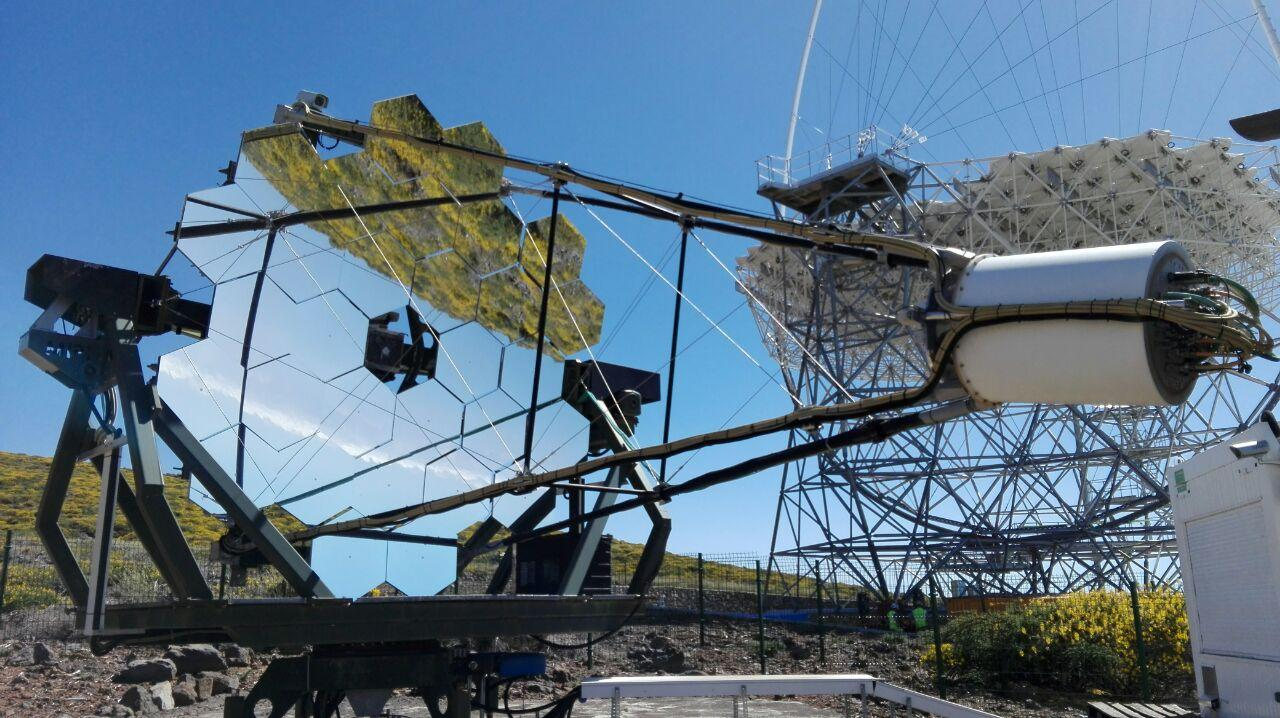
\includegraphics[width=\textwidth]{Plots/fact.jpg}
  \label{fig:fact}
  \caption{The First G-APD Cherenkov Telescope on the Observatory on the Roque des los Muchachos on the island of La Palma. Image courtesy of Kevin Schmidt.}
\end{figure}
%
The First G-APD Cherenkov Telescope \cite{FACT-Design} (FACT) is an IACT
protoype located $\SI{2200}{\metre}$ above sea-level on the Canary island of La
Palma. It measures air-shower-photons from cosmic gamma-rays with energies from
several hundred GeV up to about $\SI{10}{\tera\electronvolt}$. FACT uses a
segmented imaging-reflector with a $\SI{9.5}{\meter\squared}$ aperture and
$\SI{4.889}{\meter}$ focal-length. Apart from monitoring bright sources of
cosmic gamma-rays, like Markarian 421 and Markarian 501, FACT is used for
demonstrating and testing the usage of new technologies in the field of IACTs.

Giving it its name, FACT uses a novel kind of detector made of so called
Geiger-mode avalanche photomultipliers (GAPD). These photomultipliers make up
the 1440 pixels of Silicon-Photo-Multipliers (SiPM), FACT uses to sense
photons. Each pixel yields about $\SI{0.1}{\degree}$ field-of-view, giving FACT
a total field-of-view of $\SI{4.5}{\degree}$. Using SiPMs instead of
Photo-Multiplier-Tubes (PMTs) differentiates FACT from other IACTs and gives it
special possibilities. SIPMs are very robust, compared to PMTs and can operate
in brighter light. This makes continuos observations even during bright moon
possible. The SIPMs furthermore have a high photon detection efficiency and
therefore the potential to replace PMTs in IACTs. FACT is sampling recorded
events with a frequency of $\SI{2}{\giga\hertz}$, giving it a very good time
resolution. With these assets, FACT is well suited for long-term monitoring of
sources, finding flares and informing the astronomic community of such.

\chapter{Machine Learning and Random Forests}
\label{ch:ML}
%
The analysis tasks described in \autoref{ch:iact} make strong use of machine
learning tools to be performed in the most efficient way. There are a lot of
different machine learning techniques that find increasingly many and
successfull applications in modern physics.

\section{Machine Learning}
%
Machine learning describes the field of applied statistics that uses computers to learn to solve certain problems. The \textit{learning} is defined by~\cite{mitchell} as: \enquote{A computer program is said to learn from experience $E$ with respect to some class of tasks $T$ and performance measure $P$, if its performance at tasks in $T$, as measured by $P$, improves with experience $E$.} There is a wide variety of different tasks this can be applied to and many performance measures. The most important preposition for well suited problems is the available experience or in this case the amount of data to learn on.

Machine learning aims at solving problems that profit from the computing power
of modern technology but are not the kind of problem to be solved by a typical
program written by a human \cite{goodfellow}. The concept is to try to
reproduce the concept of intelligence within a computer.

\subsection{The Experience}
%
To make a generic machine learning algorithm work for a specific task it has to
be \textit{trained} on data. Just like a human, it needs to be given
information to base a decision on and to be shown how that decision based on
the information is supposed to look. The kind of data suitable for learning
depends on the kind of algorithm to be used and vice versa. Generally, machine
learning algorithms can be divided into \textbf{supervised} and
\textbf{unsupervised} algorithms, but in this work only supervised algorithms
will be used.

Data to derive experience from for supervised algorithms consists of data points
with a certain feature set and a specific label or true value. The datasets for
the \textit{separation} of two classes for example contain a certain feature
set for every data point and a label for the corresponding class each of these
points belongs to. Unsupervised learning therefore aims at learning to predict
a certain target value (or multiple) from a given feature set including this
value. The used learning data in this analysis is provided by simulations, so
that the true values for the machine learning tasks are known.

\subsection{The Task}
%
The task a machine learning algorithm is supposed to do is the solution of a
specific problem in the best possible way. To reach this solution the process
of learning is used but not the task. A machine learning algorithm used to
distinguish between to things is therefore given the task to distinguish two
things rather than to learn to distinguish these two. The three desired tasks
within the analysis of Cherenkov images are the \textit{separation} of
gamma-rays from hadronic cosmic rays, as well as the \textit{estimation} of the
energy and source position of cosmic gamma-rays. The kind of task already
determines what machine learning techniques are best to be used or which ones
don't suit the task and how working architectures have to look. A classification like the separation

\subsection{The Performance Measure}
%
As described above machine learning is about improving on certain tasks.
Therefore it is essential to quantify the performance during but also after the
learning process. This already implicates that performance measures are very
specific to the task. The performance of a classification task is naturally
measured by the \textbf{accuracy} of the model, because it simply describes how
many of the model's outputs are correct. When validating continuous outputs
rather than discrete classifications an accuracy is not appropriate. The
estimation of the energy, e.g., requires a continuous-valued metric.

The models are trained on specific, simulated data but only to be applied on
datasets they have \textit{not} been trained on. Thus, the interesting metrics
are those calculated on datasets complementary to the training data sets,
because they resemble the real use case. To do so, the whole dataset is divided
into a fraction determined for training and a test set on which the metrics can
be calculated. A frequently used method for this is the
\textbf{cross-validation}. The data set is divided into $n$ equaly sized, random
subsamples; $n-1$ samples are used for training whereas the single excluded
sample is used for validation. This is done $n$ times for each one of the
subsamples and the metrics calculated as the mean value of all the single
validations.

\section{Random Forests}
%
One of the most frequently used machine learning algorithms and the one used
for the tasks in this analysis is the so called random forest. This is a
supervised learning algorithm based on the so called \textit{decision tree}.

\subsection{Decision Trees}
%
Decision trees classify data points based on consecutive binary decisions. The
decisions are based on the single features of the data point and result in a
point specific result that is being returned. The number of single binary
decisions (also called \textit{leaf}) preceding the final classification is
called \textit{depth} of the tree. Decision trees are trained on labelled data
and determine thresholds for every feature to classify the data point.
%
\begin{figure}[H]
  \centering
  \begin{tikzpicture}[node distance = 3cm, auto]
    \node (f1) [feature] {\texttt{feature\_1}};
    \node (f2) [feature, below of=f1, xshift=-2.4cm] {\texttt{feature\_2}};
    \node (f3) [feature, below of=f1, xshift=2.4cm] {\texttt{feature\_3}};

    \node (c1) [class1, below of=f2, xshift=-1.2cm] {\texttt{class 1}};
    \node (c2) [class2, below of=f2, xshift=1.2cm] {\texttt{class 2}};

    \node (c3) [class1, below of=f3, xshift=-1.2cm] {\texttt{class 1}};
    \node (c4) [class2, below of=f3, xshift=1.2cm] {\texttt{class 2}};

    \draw [pil] (f1) -- node[anchor=east] {$\mathbf{>15}$\;} (f2);
    \draw [pil] (f1) -- node[anchor=west] {\;$\mathbf{\leq15}$} (f3);
    \draw [pil] (f2) -- node[anchor=east] {$\mathbf{<100}$\;} (c1);
    \draw [pil] (f2) -- node[anchor=west] {\;$\mathbf{\geq100}$} (c2);
    \draw [pil] (f3) -- node[anchor=east] {$\symbf{<-\sfrac{\pi}{2}}$\;} (c3);
    \draw [pil] (f3) -- node[anchor=west] {\;$\symbf{\geq-\sfrac{\pi}{2}}$} (c4);
  \end{tikzpicture}
  \caption{Example sketch of a decision tree. The tree decides whether an input data point is of class 1 or class 2. The available features are \texttt{feature\_1}, \texttt{feature\_2} and \texttt{feature\_3}. This decision tree has a depth of 2 and solves the task of a binary separation at each leaf (green boxes). The decision thresholds are written next to the respective connecting lines.}
  \label{fig:tree}
\end{figure}
%
To determine the best decision threshold for each leaf, a performance measure
for the information gain is necessary. For a classification task the required
metric would be the accuracy. The thresholds are thus optimized to get the best
accuracy at the respective leaf. This way the decision tree is build from the
top leaf downwards until a perfect classification is achieved or until a set
maximum depth is reached.

Decision tress can also be used for regression tasks. The only difference when
solving such tasks is the metric to find the best thresholds at each leaf.
While for classification tasks the accuracy is the natural choice, regression
tasks require a metric describing the error of the single result. Thus, the
thresholds are determined by minimizing the variance of the target variable.

\subsection{Random forests}
%
A decision tree that is fitted to the data too extensively will reach
very high accuracies, but will suffer from a very bad generalization. At some
point the tree starts to adapt to the training data's specifics too much and
won't work on other data that does not have these specific characteristics.
This phenomenon is called \textit{overfitting} and generally is represented by
a large gap between training and test errors \cite{goodfellow}. A way to
prevent this from happening is to constrain the complexity of the decision tree
while using a large number of different trees. This way the trees are not
overfitted but the complete model is still complex enough.

Random forests are generated by a process called
\textit{bagging}~\cite{bagging}. Every tree within the forest is trained on a
subset of the data randomly sampled with replacement. This way, a large number
of slightly different trees is generated. While every single decision tree is
still prone to overfitting to noise in its respective dataset, averaging over
all of them is not, as long as the trees are not correlated. To prevent such
correlations and further generalize the model, additionally every decision node
inside a single tree is only given a random subset of all available features.
Random forests therefore have two parameters: the number of trees $n$ and the
number $k$ of available features at each node.

The output of the model consisting of such a forest is then generated
by counting trees with a specific decision. A confidence for a multi-class
separation, e.g., can be generated by counting the fraction of trees that
decided for the specific class. By setting a threshold on the confidence
classification decisions can be performed. In case of regression tasks the
output of the forest is the mean of the regression results of the single trees.

\section{Performance Measures}
%
As mentioned earlier, the right performance measure depends on the task to be
validated. Since there are several different tasks to be performed during this
analysis a number of performance measures is needed for the evaluation.

\textbf{Accuracy.} The accuracy of a model describes the proportion of input
examples for which the model computes the right output. This performance
measure can be used for models with discrete outputs, such as classifications
because it only takes perfect matches as the right output.

\textbf{Receiver Operating Characteristic.} For every classification task the
so called \textit{receiver operating characteristic} curve (ROC) can be
determined. For a given class this represents the rate of correctly classified
examples dependant on the rate of falsely classified ones. The area under this
curve (AUC) can be used to quantify the performance of a classification model.
When randomly deciding on an equally distributed dataset of two classes, the
AUC is expected to be about \num{0.5}, representing the worst possible
classification performance. A perfect classification yields an AUC of \num{1}.

\textbf{Confusion Matrix.} The confusion matrix shows the results of a machine
learning algorithm against the true values. It therefore shows how well the
algorithm performs by showing where mismatches occur and with what effect. For
classifications this matrix shows what classes are most frequently confused
with each other, while for a regression task it shows how big the spread of
reconstructed values is.

\textbf{Precision.} For a classification the precision describes the fraction
of events correctly classified as signal events over all events labelled as
signal events.
%
\begin{equation}
  \text{precision} = \frac{T_{\text{p}}}{T_{\text{p}} + F_{\text{p}}}
\end{equation}
%
\textbf{Recall.} The recall of a classification model describes the fraction
of events correctly classified as signal events over all true signal events.
%
\begin{equation}
  \text{recall} = \frac{T_{\text{p}}}{T_{\text{p}} + F_{\text{n}}}
\end{equation}
%
\textbf{$F_\beta$ score.} The $F_\beta$ score of a classification model describes the harmonic mean of the precision and recall.
%
\begin{equation}
  F_\beta = (1 + \beta^2)\frac{\text{precision} \cdot \text{recall}}{\text{precision} + \text{recall}}
\end{equation}
%
\textbf{$\symbf{R^2}$ Score.} This metric quantifies the goodness of fit for a
chosen model. For a regression task, the $\symbf{R^2}$ score or sometimes
called \textit{coefficient of determination} measures how well the input data
points are approximated by the model. A regression perfectly describing the
input data is indicated by an $\symbf{R^2}$ score of 1, whereas an
$\symbf{R^2}$ score of \num{0} characterizes the opposite.

\chapter{Representing IACT data}
%
IACTs aim at reconstructing the energy, source position and particle type of
cosmic rays via their Cherenkov-light. The Cherenkov-light flashes that are
only nano seconds in duration are measured and can be separated from background
light from stars or ambient light by their brightness and topology within the
camera image. There are different ways to represent air shower data. FACT uses
the so called main-pulse representation, whereas this work focuses on a novel
data format, both of which are described in the following chapter.

\section{The Main-Pulse representation}
%
Data taken by an Imaging-Air-Cherenkov-Telescope
(IACT), like FACT, is usually represented in so called time series.
These time series owe their name to the fact that they represent voltages at the photosensors over time. Within these time series lie so called main-pulses that represent the increased voltage that a charge deposition of an air-shower causes. So by looking for those main-pulses, shower events can be found upon the detector noise and ambient light in the camera. Of course, the main-pulses consist of multiple photon signals and noise superposed over time, but in this state they are electric pulses representing the response of very specific hardware. So rather than measuring physical properties, this means that the charge deposit has to be interpretated to be transferred into physics observables, independent of these specifics \textcolor{red}{(which ones?)}. Such interpretations always include assumptions of physical and technical kinds. By integrating the charge in one pixel an equivalent of a photon count can be obtained, called the \textit{photon equivalent} (PE). So the first observable in this representation is the PE which corresponds to the best estimate of the number of photons measured per pixel. The photon counts are spatially located by the corresponding pixel they are assigned to. The 1440 pixels of FACT are the determining grid that yield the spatial coordinates of every shower event.

The second observable is the time. When the telescope is triggered and records
data the arrival time of the event is measured via the time information within
the time series. From the time series a quantized timing information per pixel
can be developed by dividing the event into time slices. From this the arrival
time of the photons per pixel can be calculated by averaging. Thus, the arrival
times $t$ per pixel are the second observable of the main-pulse event
representation, besides the photon-equivalents.

\begin{figure}
  \begin{subfigure}{0.475\textwidth}
    \includegraphics[width=1.1\textwidth, page=40]{Plots/cleaning_facttools_pe_20131104_162.pdf}
  \end{subfigure}
  \begin{subfigure}{0.475\textwidth}
    \includegraphics[width=1.1\textwidth, page=40]{Plots/cleaning_facttools_arrival_times_20131104_162.pdf}
  \end{subfigure}
  \caption{The measured observables of the main-pulse representation are shown as scatter plots within the pixels \textcolor{red}{[source]}. On the left the distribution of photon-equivalents $c$ of a typical shower event (Crab observation on November, 4th 2013, run 162, event 80) is shown. On the right the arrival times of that event's photons with respect to the mean arrival time in ns are displayed.}
  \label{fig:mainpulse}
\end{figure}

\section{The PhotonStream representation}
\label{sec:phs}
%
The PhotonStream representation aims at creating a data format consisting of photons by storing their observed physical properties \textcolor{red}{(klarmachen, dass auf Sebastian's Arbeit basierend)}. So from the measured time series single photons are extracted instead of deriving photon counts in pixels. Each of these photons is assigned an arrival time and pixel, creating a list of arrival times per photon for each pixel. By doing so, a 3-dimensional data set is created, which can be represented in form of so called point clouds (\autoref{fig:point_cloud}).
%
\begin{figure}
  \centering
  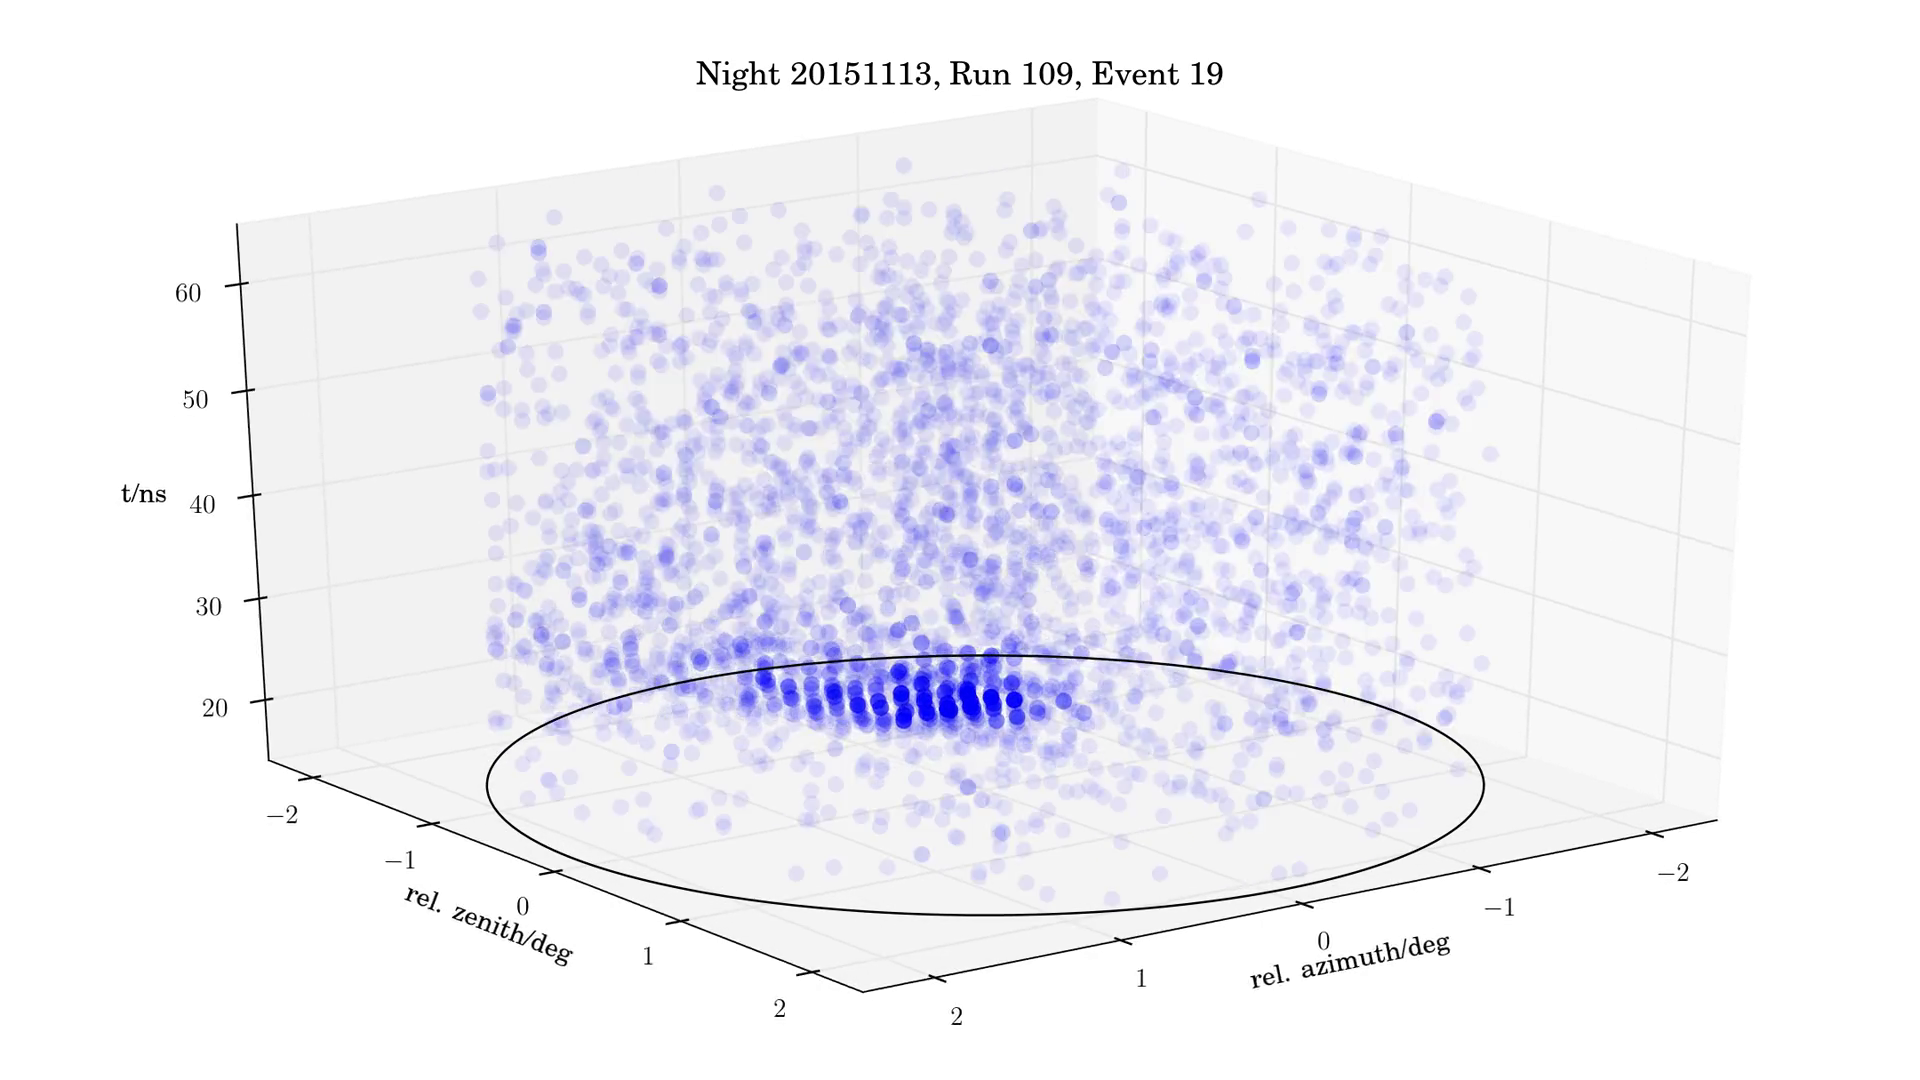
\includegraphics[width=0.7\textwidth]{Plots/event2.png}
  \caption{Uncleaned event represented by the 3-dimensional point cloud of the Photonstream. Every blue sphere represents a measured photon in the corresponding time slice and pixel.}
  \label{fig:point_cloud}
\end{figure}
%
\subsection{Single Photon Extraction}
%
To generate the PhotonStream data from the measured time series, single photons
need to be found and extracted. FACT is sampling recorded events with a
frequency of $\SI{2}{\giga\hertz}$. This yields a very high time resolution, but still quantized values within the time series. The time series consists of multiple signals
of single photons and different kinds of noise. Among the latter are several
electronic artifacts. The photon extraction does not take such artifacts into
account, so the data has to be cleaned of those at first. Unfortunately there
are rare kinds of artifacts that can not be handled and may remain in the
calibrated data.

The transformation of data to the PhotonStream consists of two steps:
%
\begin{enumerate}
  \item find single photons and determine their arrival times
  \item subtract those photons from the time series until only noise is left
\end{enumerate}
%
To achieve this two templates are used. At first, the ideal template of a
single photon pulse $T_1$ is generated. It represents the discharge-pulse of a
GAPD when measuring a photon. This template is used to subtract found photons
from the remaining time series. To find these pulses the rising edge of that
template is used. This template $T_2$ represents the first
$\SI{10}{\nano\second}$ of $T_1$.

To extract all photons from a time series an iterative algorithm is used, that
finds rising edges of single photons and then extracts the full photon pulse
$T_1$. An example is shown in \autoref{fig:extraction}. Red vertical lines
indicate the time position of a found rising edge template $T_2$. The time
series of a single pixel is correlated with $T_2$ to find the maximum of that
correlation. The response is defined as
%
\begin{equation}
  R[t] = A_\text{pixel}[t]\cdot T_2[t] \, .
\end{equation}
%
The maximum of the response is identified as the arrival time of a photon pulse.
After such a pulse has been found, the full photon pulse template $T_1$ is
subtracted. The remaining time series is then searched for further photon
pulses until only noise is left. The stopping-criterion defining the last
iteration step is reached when the maximum of the response $R[t]$ drops below
half of the maximum of the response to a single-pulse.
Every found arrival time of a photon is written to a list containing the
PhotonStream for the specific event and pixel.
%
\begin{figure}
  \centering
  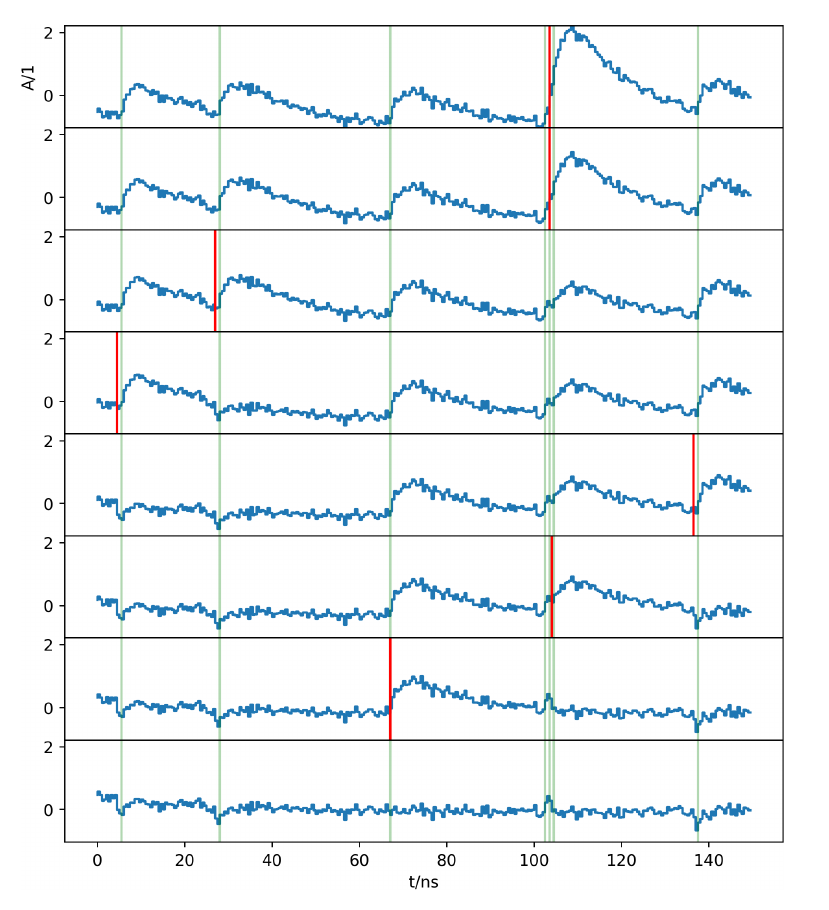
\includegraphics[width=0.95\textwidth]{Plots/photon_extraction_sebastian.png}
  \caption{Example of the photon extraction from a calibrated time series \textcolor{red}{[source]}. Shown are several steps of the iterative extraction for the time series of a single pixel. The top frame shows the full time series as returned from the calibration process. The red vertical line shows the time position of the first found photon. After subtracting the photon pulse template $T_1$, the series as shown in the frame below remains, where another photon is found at the same position (red vertical line). The extraction continues until the time series in the bottom frame remains, which is considered noise. The extracted photon arrival times represent the PhotonStream for this specific pixel.}
  \label{fig:extraction}
\end{figure}
%

\chapter{Analysis chain}\label{ch:analysis}
%
For the PhotonStream data representation, as a new way of describing IACT data,
there is no reference analysis chain so far. The new possibilities of this
representation need new analysis structures and give way for new methods and
solutions. This work is therefore comparing different approaches derived from classical analysis chains used by the FACT collaboration to solve the
tasks of this analysis. A schematic representation of the analysis flow is
shown in \autoref{fig:analysis}.
%
\begin{figure}[H]
  \centering
  \begin{tikzpicture}[node distance = 1.5cm, auto]
    \node (f1) [feature, xshift=-2.0cm] {PhotonStream};
    \node (f2) [LP, xshift=2.0cm] {Largest Pulse};
    \draw[line width=0.7mm, below of=f1] (-4.2,0.7) -- (4.2,0.7);
    \node (s1) [astep, xshift=-4.0cm, anchor=west, below of=f1] {calibration};
    \node (f3) [feature, below of=f1] {\begin{varwidth}{9em}\centering{Extracting single photons}\end{varwidth}};
    \node (f4) [LP, below of=f2] {\begin{varwidth}{9em}\centering{Identifying large pulses}\end{varwidth}};

    \node (f5) [feature, below of=f3] {\begin{varwidth}{9em}\centering{density-based clustering}\end{varwidth}};
    \node (f6) [LP, below of=f4] {\begin{varwidth}{9em}\centering{pixel-based thresholds}\end{varwidth}};
    \node (s2) [astep, below of=s1] {image cleaning};
    \node (f7) [feature, below of=f5] {parameter set A};
    \node (f8) [LP, below of=f6] {parameter set B};
    \node (s3) [astep, below of=s2] {parametrization};
    \node (f9) [both, below of=f7, xshift=2.0cm] {AICT Tools~\cite{aicttools}};
    \node (s4) [astep, below of=s3] {separation};
    \node (f10) [both, below of=f9] {AICT Tools~\cite{aicttools}};
    \node (s5) [astep, below of=s4] {energy \& origin reconstruction};

    \draw [arrg] (f3) -- node[anchor=east] {} (f5);
    \draw [arrg] (f3) -- node[anchor=east] {} (f6);
    \draw [arry] (f4) -- node[anchor=east] {} (f6);
    \draw [arrg] (f5) -- node[anchor=east] {} (f7);
    \draw [arrg] (f6) -- node[anchor=east] {} (f7);
    \draw [arry] (f6) -- node[anchor=east] {} (f8);
    \draw [arrg] (f7) -- node[anchor=east] {} (f9);
    \draw [arry] (f8) -- node[anchor=east] {} (f9);
    \draw [arry, color=cyan] (f9) -- node[anchor=east] {} (f10);
  \end{tikzpicture}
  \caption{Schematic flow of the different analysis steps of this analysis. The PhotonStream analysis uses different calibrations (\autoref{sec:phs}) and a different cleaning (density-based clustering) than the LP representation. Nonetheless, the PhotonStream data contains all information neccessary to apply the LP pixel-based threshold cleaning on the calibrated data.}
  \label{fig:analysis}
\end{figure}
%
To generate PhotonStream data a different calibration is needed. As described
in \autoref{sec:phs}, instead of finding large pulses and calculating the data
coordinates, the time series data is turned into single photons. The additional
information of the PhotonStream is then used to clean the image in the
three-dimensional spacetime via the DBSCAN algorithm (\autoref{subsec:dbscan}), rather than by setting
timing and PE thresholds for air-shower pixels. Nonetheless, the PhotonStream
data contains all that is neccessary to perform this pixel-based cleaning
instead. Therefore, this analysis is investigating said cleaning on
PhotonStream data as well as the DBSCAN cleaning. The parametrization of the
events in PhotonStream representation uses a subset of the features of the LP
analysis, to have the best comparability. Especially the additional timing
information of the PhotonStream is not used in feature generation for this
analysis. The different analysis steps shown in \autoref{fig:analysis} are
described in the following section. The results of the combinations of these
steps as represented by the arrows in \autoref{fig:analysis} are then evaluated
in \autoref{ch:results}.

\section{Image Cleaning on the PhotonStream}\label{sec:phs_clean}
%
As pointed out in \autoref{ch:iact} the Cherenkov-light of air-showers shows a
very specific topology. The emitted photons are coherent in space and time:
they originate from a single very high energetic and therefore very fast
primary particle and thus appear in a very brief time window of a few
nanoseconds. Furthermore, the characteristic Cherenkov-angle under which the
light is emitted, creates a light cone, which, when projected to the
$x$-$y$-plane of the camera causes the specific elliptical shape. Both of these
topological features are mandated by the physical process and can therefore be
used for the cleaning. Background events like ambient light or
starlight do not show these characteristics and tend to appear randomly.

The three-dimensional $xyt$-representation of the PhotonStream, called point cloud, quantifies photons with exactly those three observables. Thus, a cleaning
within the three-dimensional spacetime can heavily use the known topology.
Within the point cloud, an air-shower will appear as a very dense cluster of
photons, surrounded by a merely isotropic distribution of background photons.
These characteristics of shower events in the PhotonStream representation
naturally suggest a density-based clustering algorithm as the cleaning method
of choice. The two challenges at hand are the choice of a suited algorithm and
a well defined metric to make the three-dimensional spacetime usable.

\subsection{Air-showers in the Point Cloud}
%
The three-dimensional spacetime of the PhotonStream and its representation as a
point cloud eventually mixes spatial dimensions with time. While this is
physically motivated, defining distances in such a space is not trivial. They
are highly dependent on the chosen metric, which defines how time corresponds to
space. This already implies that the choice of metric contains certain
assumptions and can be adapted to specific preferences. It also shows that the
image characteristics, its cleaning and therefore all analysis steps are
influenced by the choice of parameters. The essential parameter
is the factor $\alpha$, which transfers time to space and vice versa:
%
\begin{equation}
  c_{t} = \alpha \cdot t \, .
  \label{eq:metric}
\end{equation}
%
The choice of this parameter e.g. gives the possibility to prefer spatial
distance over timing information, or the opposite. The spacetime of the
point cloud is quantized in all its three dimensions: the pixels of the camera
define the spatial grid, whereas the time slices, each event is binned to, do so
for the timing information. When trying to separate air-showers from
background via the density of the shower's photons, the distance between photons plays the
essential role. The natural way to equalize between space and time is to adapt
to the photon distribution of a typical air-shower along each dimension. So, by
choosing
%
\begin{equation}
  \alpha = 0.35\cdot10^9\,\si{\degree\per\second}\, ,
\end{equation}
%
the one-dimensional density distribution of photons along the coordinates
$c_x$, $c_y$ and $c_t$ is the same. With this metric, the distance between two
photons $a$ and $b$ is defined as
%
\begin{equation}
  d_{a,b} = \sqrt{(c_x^a - c_x^b)^2 + (c_y^a - c_y^b)^2 + (c_t^a - c_t^b)^2}
\end{equation}

The two-dimensional projections of the point cloud within this metric are shown
in \autoref{fig:pc} for an example air-shower event. With the calculated
degree-equivalent of time the air-shower shows a similar distribution in
each dimension. Air-shower events show high density regions represented by
dark blue photon accumulations in this point cloud representation.
%
\begin{figure}[H]
  \centering
  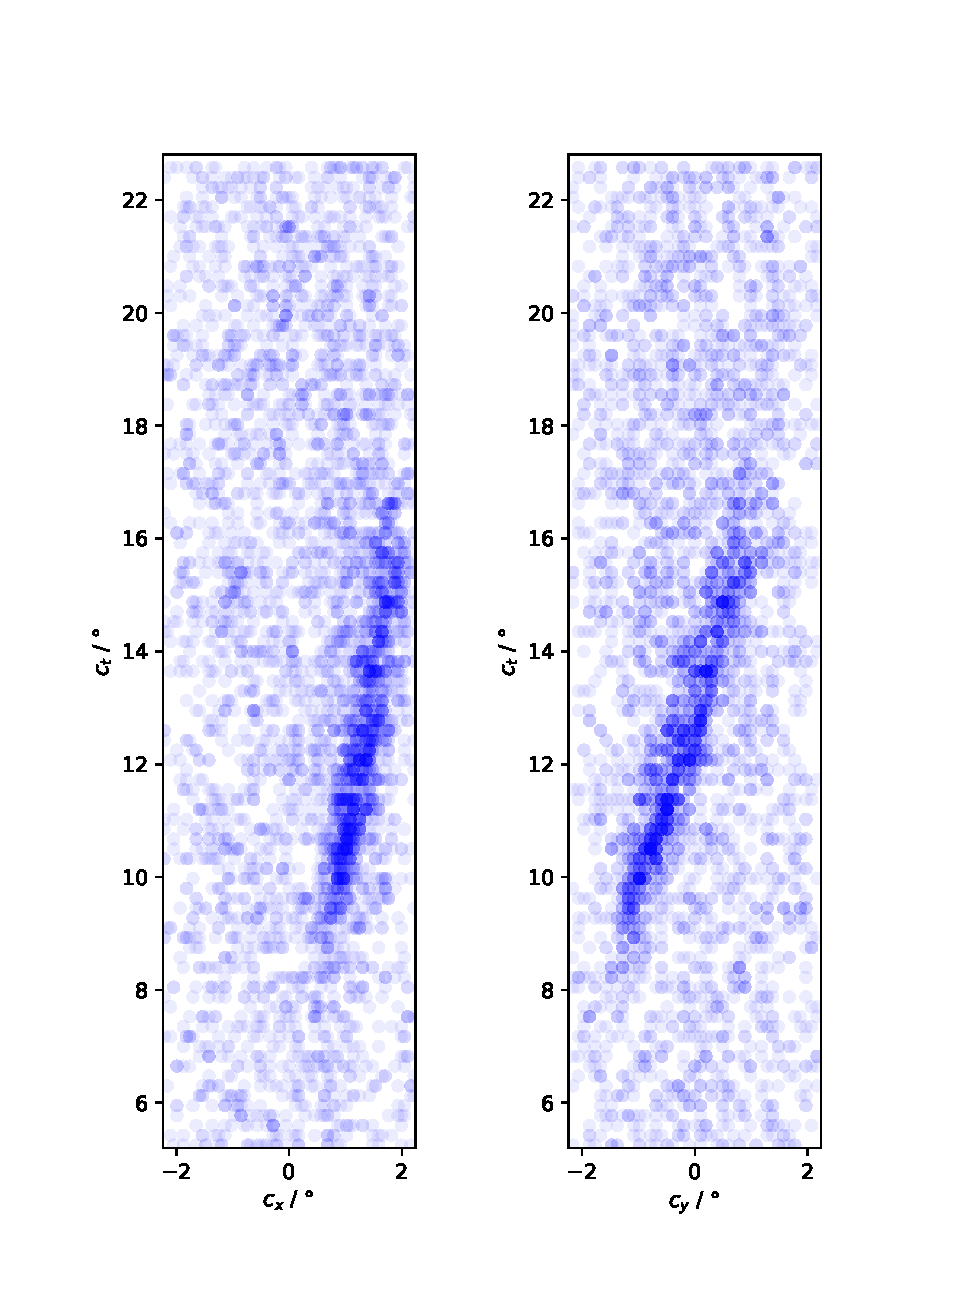
\includegraphics[width=0.6\textwidth, angle=-90]{Plots/point_cloud.pdf}
  \caption{Two-dimensional projections of the point cloud using the metric described above. The blue spheres represent single photons. Dense regions therefore appear in a darker blue.}
  \label{fig:pc}
\end{figure}
%

\subsection{Density-based Clustering with DBSCAN}\label{subsec:dbscan}
%
To find clusters of photons within the space described above, the PhotonStream
uses the \textit{density-based algorithm for discovering clusters with noise}
(DBSCAN) \cite{DBSCAN}. The DBSCAN is well suited for finding air-showers with the PhotonStream's observables, when choosing the right parameter set for the algorithm. This unsupervised algorithm either assigns each extracted photon to one of potentially multiple
clusters or identifies it as a night-sky-background photon. There are no
assumptions on the shape, location or number of the clusters. The algorithm is
characterized by only two parameters.
%
\begin{description}[]
  \item[m] the minimum number of photons to make up a cluster
  \item[$\symbf{\varepsilon}$] the maximum distance between two photons to be considered dense
\end{description}
%
These two parameters represent the specific topology of the air-shower events
by giving limits on typical shower sizes and spreads in spacetime. For
air-shower events recorded by FACT the best choice was found to be $m = 20$ and
$\varepsilon = \SI{0.45}{\degree}$ \cite{sebastian}. So, to survive the cleaning, every found
cluster must at least contain 20 photons within a maximum distance of
$\SI{0.45}{\degree}$ to the respective closest photon. The algorithm determines
the clusters by iterating over the photons in 4 steps:
%
\begin{enumerate}
  \item loop over photons until a dense region with at least $m$ photons is found
  \item add photons to the newly found cluster that are within distance $\varepsilon$ or connected via a chain of dense photons
  \item if nothing to add to cluster restart 1. with leftover photons
  \item mark all photons not assigned to any dense cluster as night-sky-background
\end{enumerate}
%
This way every photon is either belonging to a cluster of an air-shower, or
discarded as background. This determination is taking place in the whole space
of observables the whole time. There are no intermediate steps, only taking
single observables into account, which very much represents a way to find
air-showers in a space well suited for describing them. Furthermore, this way
single photons are selected rather than specific pixels. When expecting
background photons also within signal pixels, this should yield a cleaned image,
closer to the true air-shower image. An example event before and after cleaning
is shown in \autoref{fig:event_u} and \autoref{fig:event_c}.
%
% \begin{figure}
%   \begin{subfigure}{\textwidth}
%     \centering
%     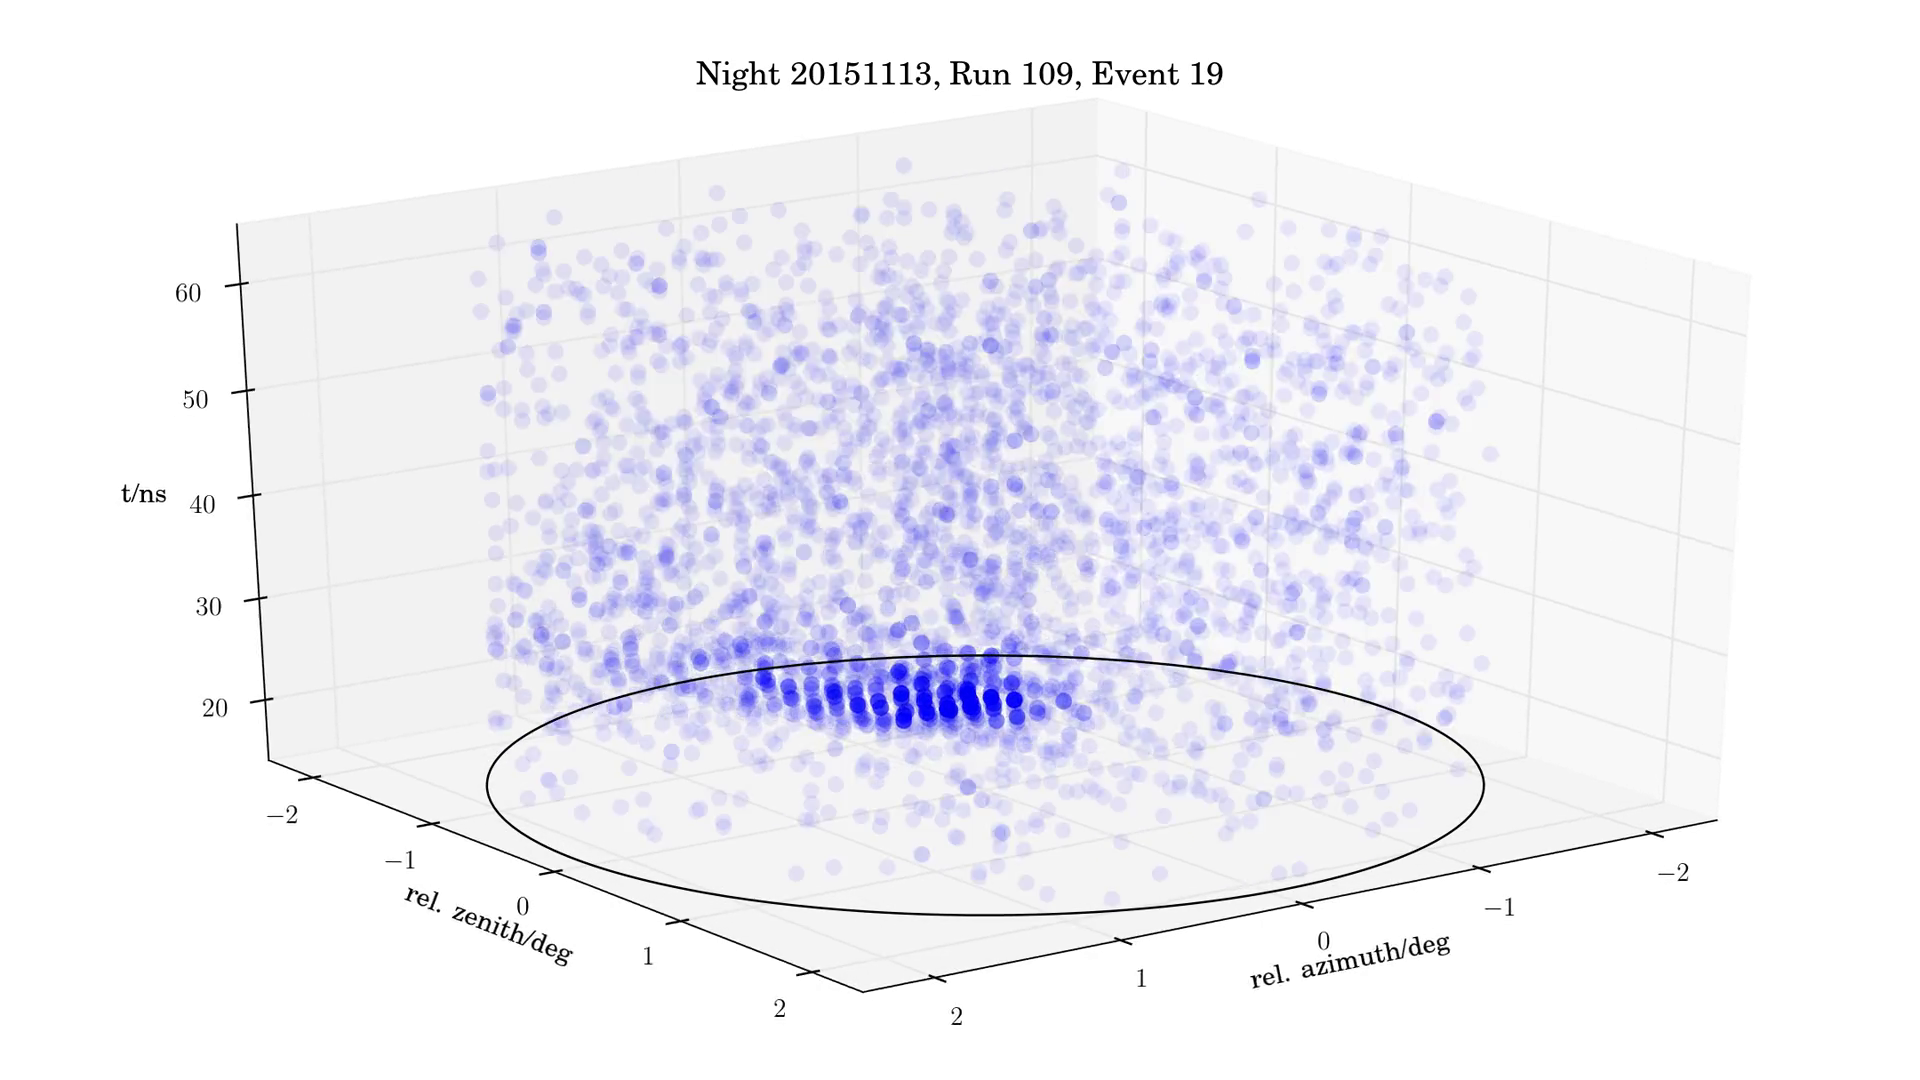
\includegraphics[width=0.9\textwidth]{Plots/event2.png}
%   \end{subfigure}
%   \begin{subfigure}{\textwidth}
%     \centering
%     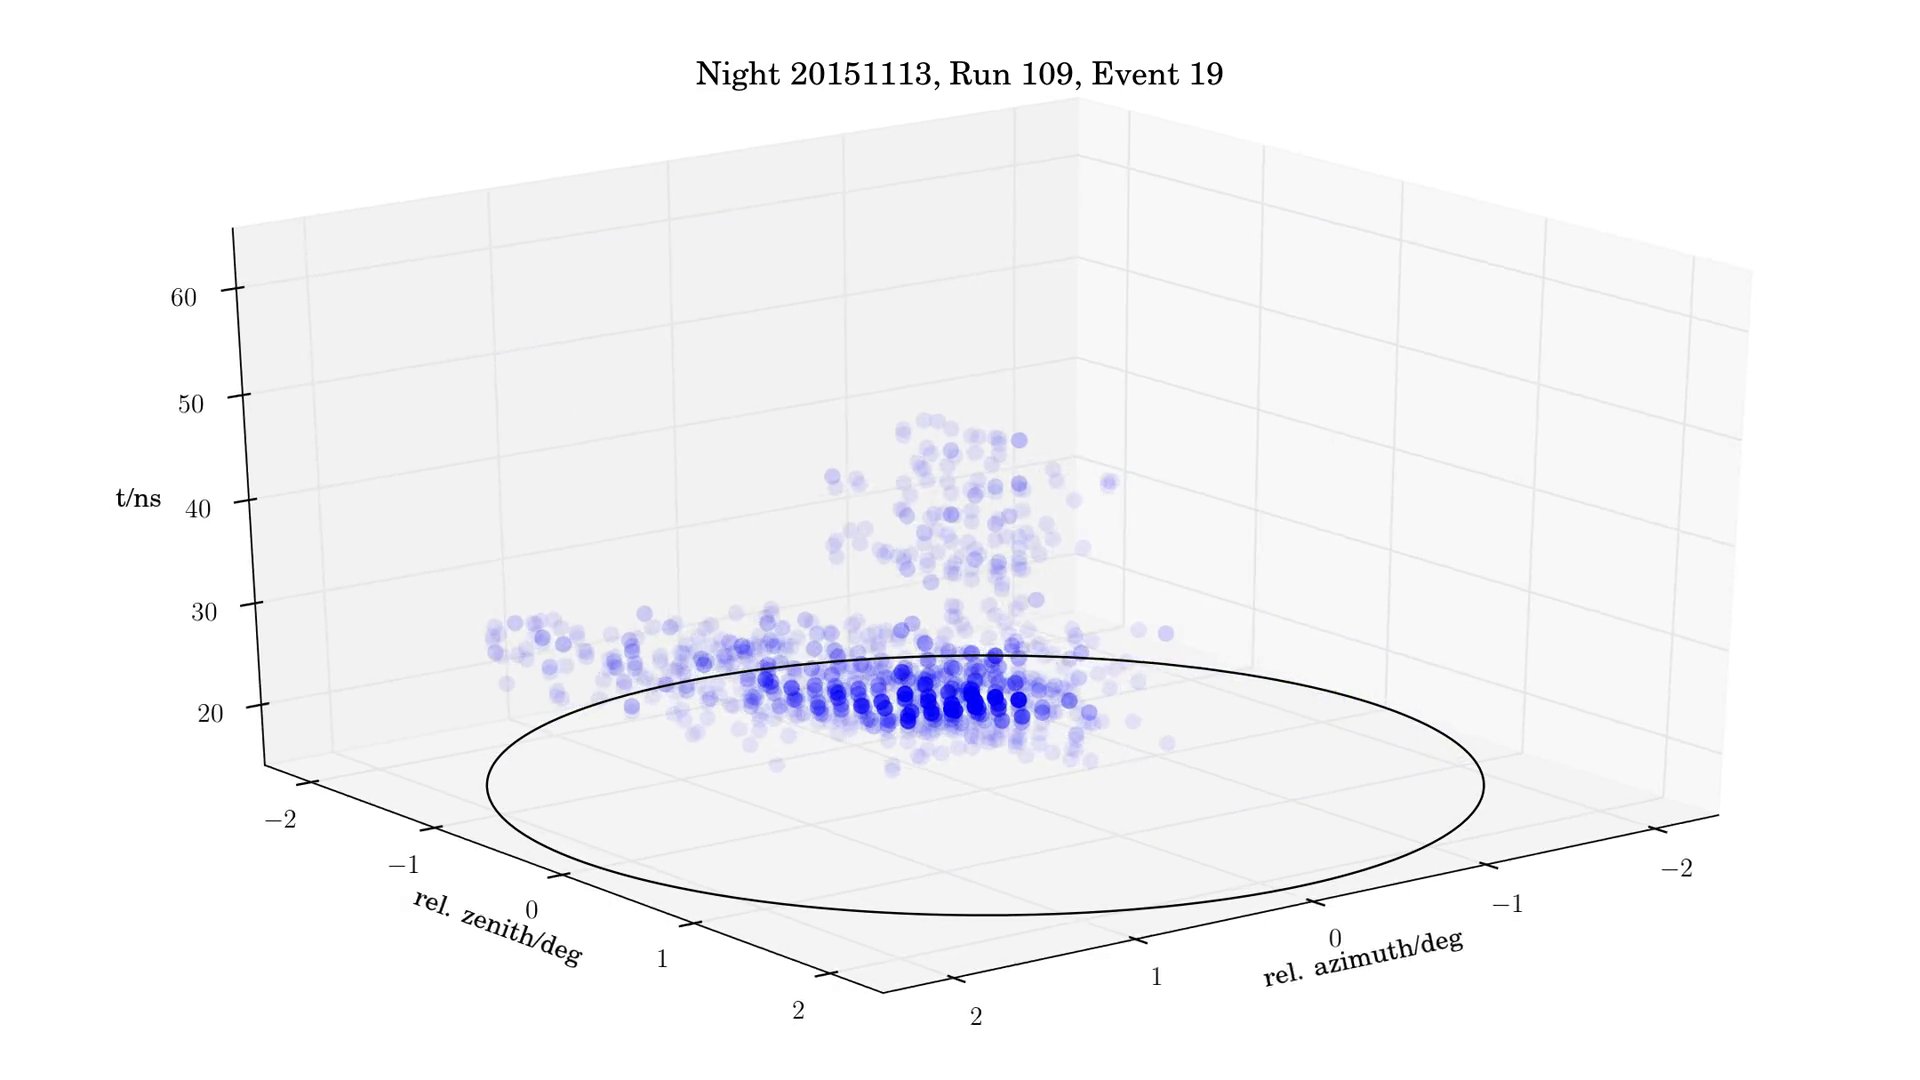
\includegraphics[width=0.9\textwidth]{Plots/event1.png}
%   \end{subfigure}
%   \caption{Event represented by the three-dimensional point cloud of the Photonstream. Every blue sphere represents a measured photon in the corresponding time slice and pixel. The right figure shows the remaining photons after cleaning.}
%   \label{fig:event}
% \end{figure}
%
%
\begin{figure}
  \centering
  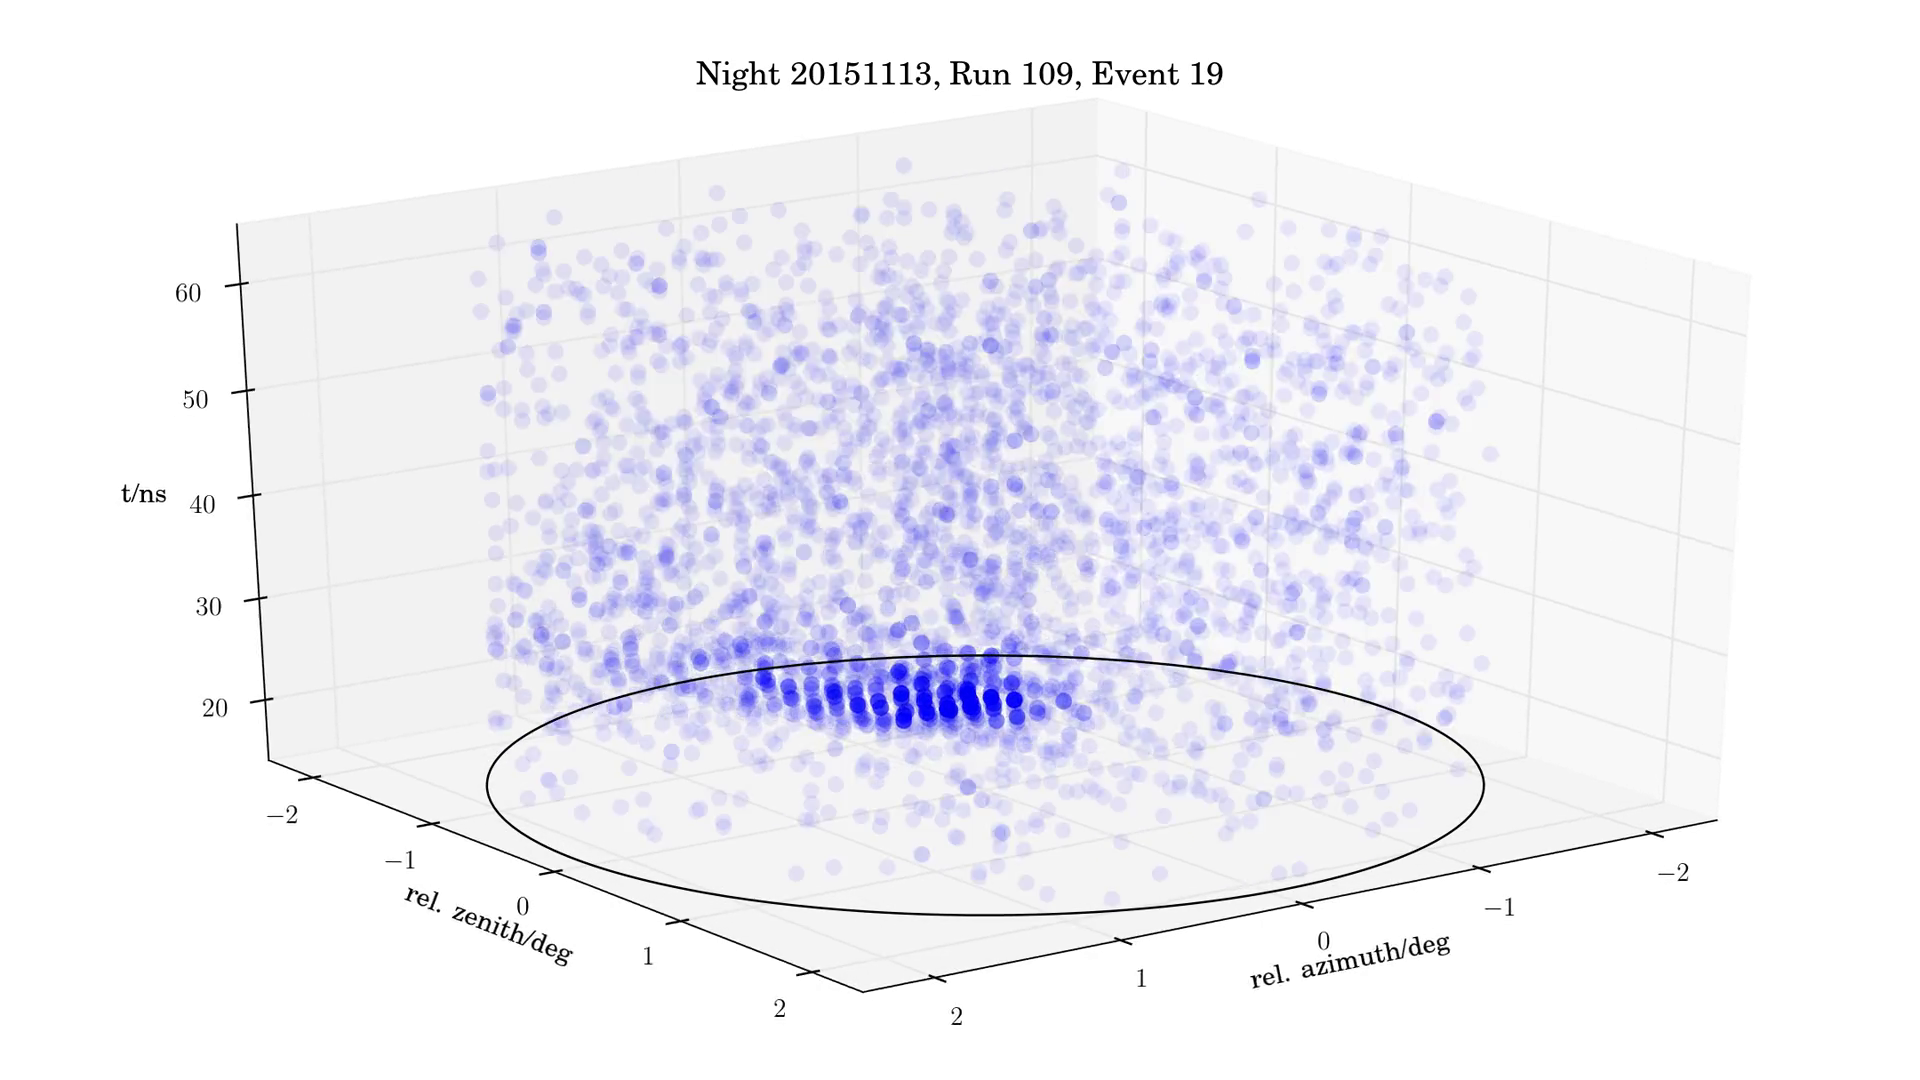
\includegraphics[width=0.85\textwidth]{Plots/event2.png}
  \caption{Uncleaned event represented by the three-dimensional point cloud of the Photonstream. Every blue sphere represents a measured photon in the corresponding time slice and pixel.}
  \label{fig:event_u}
\end{figure}
\begin{figure}
  \centering
  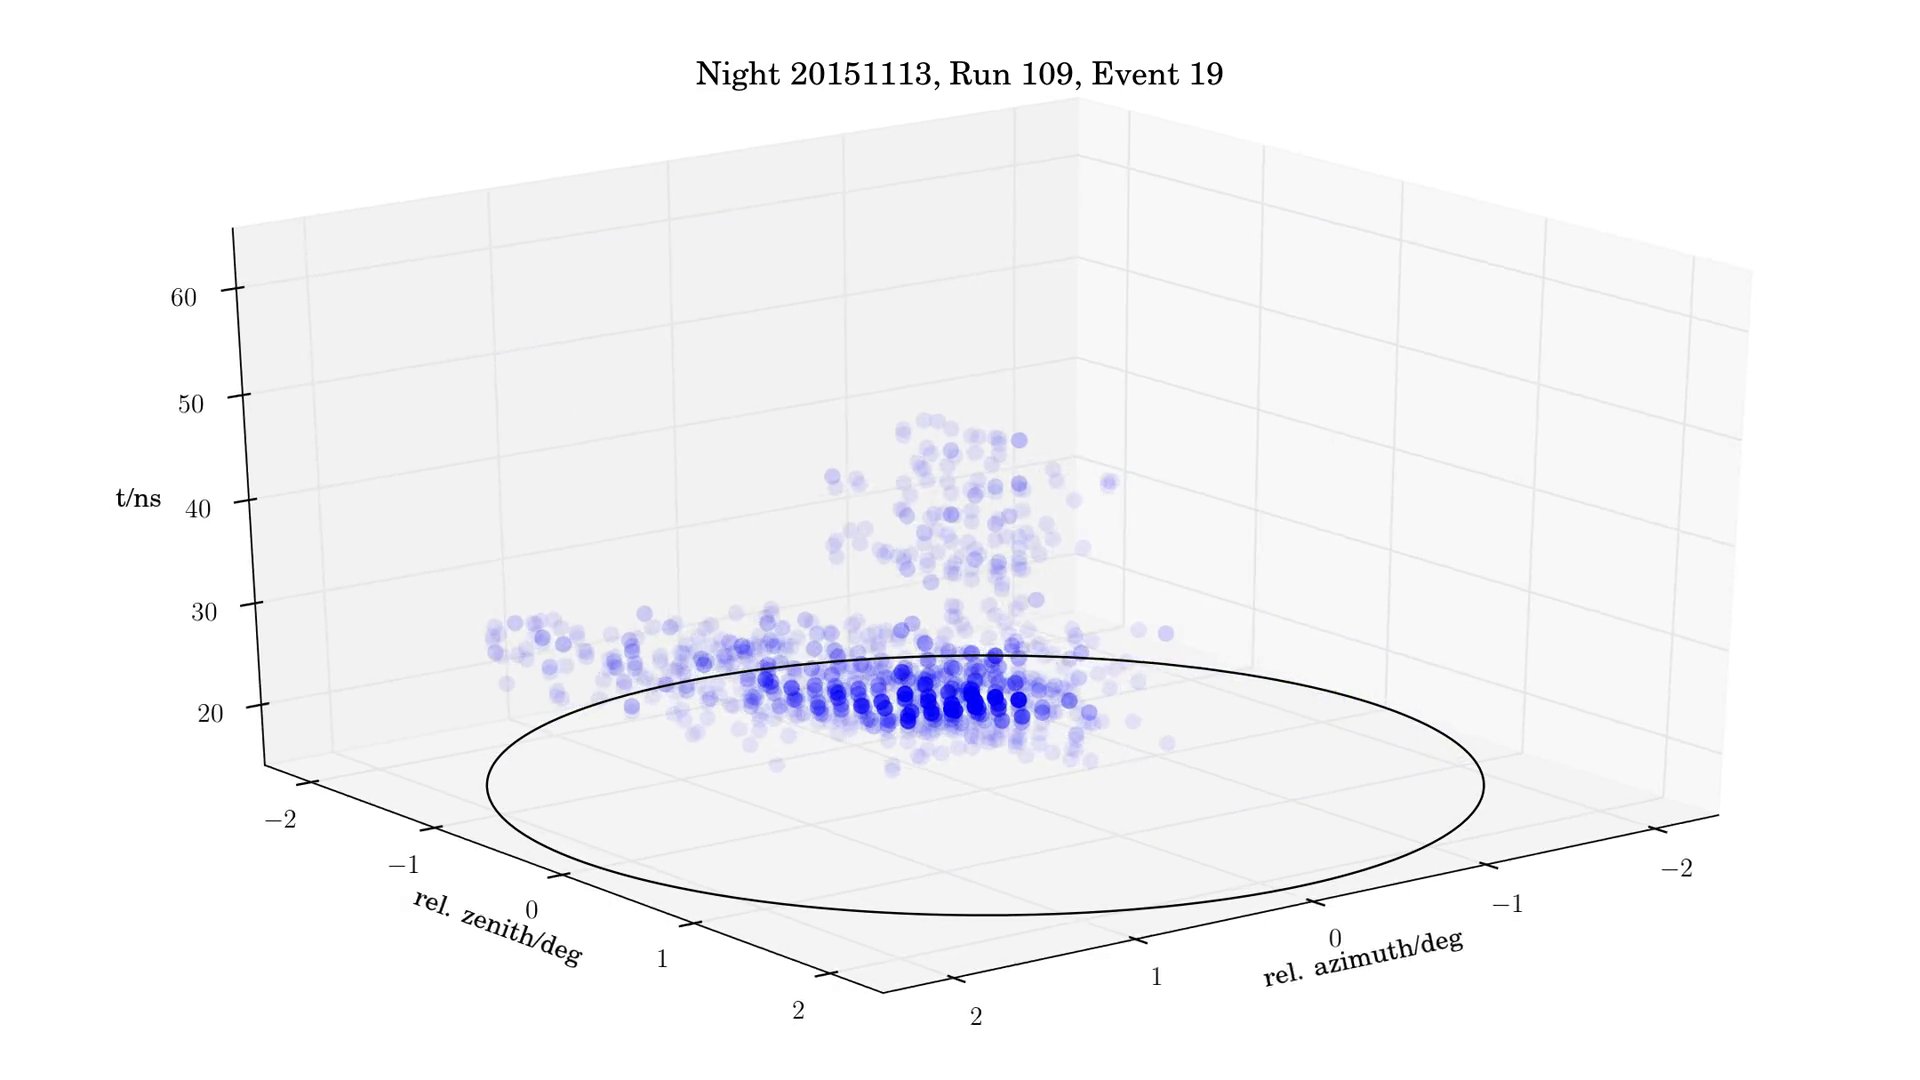
\includegraphics[width=0.85\textwidth]{Plots/event1.png}
  \caption{Cleaned event represented by the three-dimensional point cloud of the Photonstream. Every blue sphere represents a measured photon in the corresponding time slice and pixel.}
  \label{fig:event_c}
\end{figure}
%

\section{Parametrization of Events}
\label{sec:params}
%
For the classical analysis the detected images need to be parametrized. The
learning algorithms work with specific features rather than the whole image,
although there are indeed ways to analyze whole images.

The parametrization that is most frequently chosen for IACT data is based on
the one proposed by Hillas~\cite{Hillas}. It operates on the two-dimensional
images recorded by the cameras, calculating features of the air-shower pixels.
In the original publication these features were used to successfully analyze
images on a 37-pixels camera. The parametrization is based on the light
distribution among the air-shower pixels by calculating the eigenvalue
decomposition of the covariance. A graphical representation of a typical
air-shower image is shown in \autoref{fig:hillas}.
%
\begin{figure}
  \centering%
  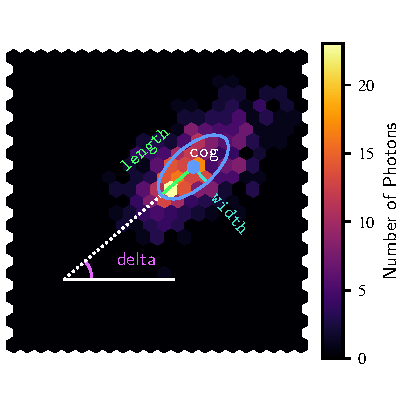
\includegraphics[width=0.6\textwidth]{Plots/hillas.pdf}%
  \caption{A graphical representation of a typical air-shower image \cite{maxhillas}. The figure shows the number of photons per pixel of an air-shower. The dotted
  line represents the air-shower axis. It corresponds to the line minimizing the
  sum of perpendicular angular distance, weighted by the number of photons per
  pixel. The standard deviations along this axis and the perpendicular axis are
  the two features called \texttt{length} and \texttt{width}. The center of
  gravity (\texttt{cog}) of the air-shower image is the two-dimensional weighted
  mean of all shower pixels.}%
  \label{fig:hillas}%
\end{figure}
%
The figure shows the number of photons per pixel of an air-shower. The dotted
line represents the air-shower axis. It corresponds to the line minimizing the
sum of perpendicular angular distance, weighted by the number of photons per
pixel. The standard deviations along this axis and the perpendicular axis are
the two features called \texttt{length} and \texttt{width}. The center of
gravity (\texttt{cog}) of the air-shower image is the two-dimensional weighted
mean of all shower pixels. The position and orientation of the shower is also
characterized by the angle \texttt{delta}. It is the angle between the shower
axis and the camera's $x$-axis. The \texttt{size} of the air-shower simply
corresponds to the sum of photons measured in all air-shower pixels.

To further parametrize the air-showers also higher order statistical moments of
the light distributions are used. Those are the third (\texttt{skewness}) and
fourth (\texttt{kurtosis}) statistical moments of the air-shower photons along
the two axes defined above. The values are calculated in a rotated system in
respective to the camera system, so that the two main axes define the
coordinate axes.
%
\begin{align}
  \text{skew}(X) &= \text{E}\left[\left(\frac{X-\mu}{\sigma}\right)^3\right] \label{eq:skew} \\
  \text{kurt}(X) &= \text{E}\left[\left(\frac{X-\mu}{\sigma}\right)^4\right]  \label{eq:kurt}
\end{align}
%
Additional to the \texttt{size} of an air-shower the number of pixels
\texttt{n\_pixel} containing air-shower photons is used as a feature. Since
there might be more than one cluster in an air-shower event, especially for
hadron showers, the ratio of the cluster sizes (\texttt{cluster\_size\_ratio})
is used for the gamma hadron separation.
%
\section{Reconstruction of the Source Position}
\label{sec:source_pos}%
%
FACT is a single telescope and therefore has no stereoscopic features to
determine the origin of the cosmic ray showers. Thus, specific techniques only
using the features of the air-shower images have to be performed. In this
analysis the so called disp-method is used. It estimates the origin position of
the cosmic gamma-rays by estimating the two features \texttt{disp} and \texttt{sign}. The two
dimensional problem of determining $x$ and $y$ coordinates is turned into a
regression task and a classification task. The estimated source position within
the camera's image is assumed to be on the shower's main axis. To find this
position the first step is to estimate the distance to the \texttt{cog} of the
air-shower. \texttt{disp} is representing that distance of the estimated source inside
the camera. As described earlier the fraction of \texttt{width} and \texttt{length} is dependent
on the angle under that the air-shower is hitting the camera. Thus, it is
\enquote{pointing} to the cosmic origin of the shower.

The second step is to determine the direction of \texttt{disp} along
the main axis. As shown in \autoref{fig:disp_amb} the distance \texttt{disp} alone is
not sufficient to determine the source position, but an additional direction is
needed. Otherwise there remains an ambiguity, as shown in the two examples.
The assumption of the origin position being on the shower axis reduces this
task to a binary classification of the sign of \texttt{disp}.
%
\begin{figure}
  \begin{subfigure}{0.5\textwidth}
    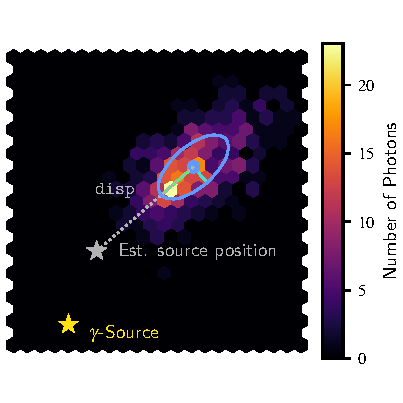
\includegraphics[width=\textwidth]{Plots/hillas_4.pdf}
  \end{subfigure}
  \begin{subfigure}{0.5\textwidth}
    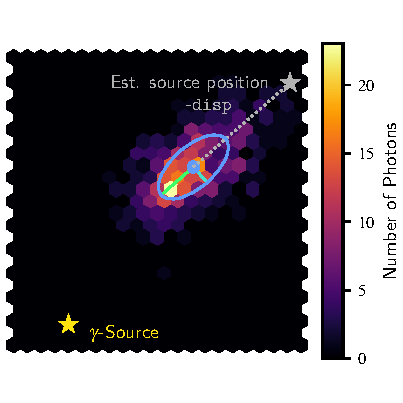
\includegraphics[width=\textwidth]{Plots/hillas_5.pdf}
  \end{subfigure}
  \caption{Ambiguity of the reconstruction direction along an example shower's main axis \cite{maxhillas}. The calculated \texttt{disp} can be applied to two directions along the shower axis and therefore needs to be determined as well.}
  \label{fig:disp_amb}
\end{figure}
%
The reconstructed source position can then be validated by comparing it to the
known source position as shown in \autoref{fig:disp}. The calculated distance
between the both is labelled $\theta$ and source specific.
%
\begin{figure}
  \centering%
  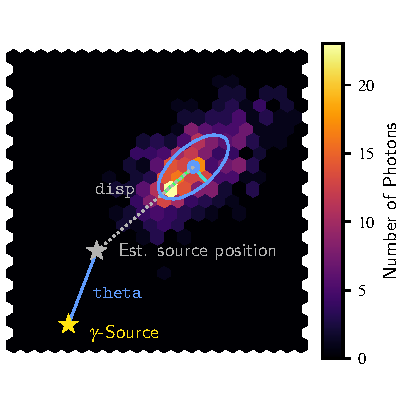
\includegraphics[width=0.6\textwidth]{Plots/hillas_disp.pdf}%
  \caption{Result of the reconstruction of the source position using the disp-method \cite{maxhillas}. From the reconstructed source position the distance $\theta$ to the true source position can be calculated to validate the reconstruction.}%
  \label{fig:disp}%
\end{figure}
%
\section{Image Cleaning with Pixel-Based Thresholds}
\label{sec:thresh}
%
When using the largest-pulse representation (LP), a different cleaning is
used. Since the PhotonStream is a different representation, of course the
optimal cleaning differs. When cleaning LP data an algorithm working on the PE
of the pixels is used. This cleaning is based on the assumption that air-shower
images contain a certain minimum number of photons per pixel and appear in a
quite small range of time and space within one event. It does not contain any
assumptions on the number of clusters per event, but with the mentioned
assumptions generally implies a certain topology within the camera's
coordinates. Since arrival times in this representation are properties per
pixel the time correlation has to be given between neighboring pixels. The
algorithm executes the following steps \cite{facttools}:
%
\begin{enumerate}
  \item find pixels containing more photons than an upper threshold $t_1$ (5~PE)
  \item remove pixels with less than 2 neighbors above $t_1$
  \item add neighbors of remaining pixels that are above a lower threshold $t_2$ (2.5~PE)
  \item remove pixels that have less than 2 neighbors arriving in $\SI{5}{\nano\second}$ time window
  \item remove single pixels with less than 2 neighbors
  \item remove pixels that have less than 2 neighbors inside a $\SI{5}{\nano\second}$ time window
\end{enumerate}
%
The remaining pixels are considered to be the cleaned image. When projecting
the PhotonStream data into a camera image and calculating the mean arrival
times per pixel, unlike in the three-dimensional space for DBSCAN, this
cleaning can equivalently be performed on PhotonStream data.


\section{Energy Estimation and Signal-Background Separation}
%
The generated features (\autoref{sec:params}) are used for the estimation of
the primary particle's energy and the classification of the particle via
machine learning algorithms as described in \autoref{ch:ML}. To generate and
train the random forests, the framework \texttt{aict-tools} \cite{aicttools} is
used. It provides executables for the configuration, training and application
of machine learning tasks on IACT data. The executables use the popular python
machine learning library \texttt{scikit-learn}~\cite{scikit-learn}, which comes
with a plethora of supervised and unsupervised machine learning algorithms,
data preparation tools and evaluation functions. All three major tasks of this
analysis can be performed by these tools on the used data set.

\chapter{The FACT Open Crab Sample}
%
This analysis is exclusively using openly accessible data \cite{fact-data}. In November 2017 the
FACT collaboration made a dataset of Crab Nebula observations public
\cite{FACT-Design, FACT-Calib}. This dataset contains $\SI{17.7}{\hour}$
of Crab Nebula observations made between November 1, 2013 and November 6, 2013.
This sample is chosen because of the good observation conditions. The Crab Nebula furthermore is the standard candle for IACT astronomy and the performance of any new instrument or analysis is best tested using this benchmark \cite{holder}. Alongside the
data Monte Carlo simulations (MC) for diffuse proton air-showers and point-like
as well as diffuse gamma ray air-showers are distributed. The observations
cover a zenith distance between $\SIrange{6}{30}{\degree}$, \autoref{fig:zenith}.
%
\begin{figure}
  \centering%
  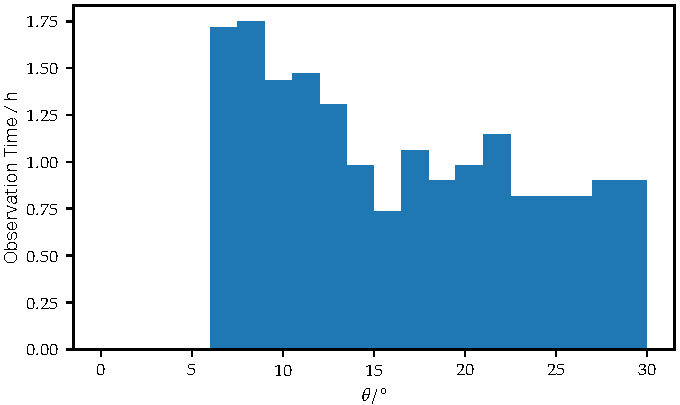
\includegraphics[width=0.8\textwidth]{Plots/zenith.pdf}%
  \caption{The distribution of the $\SI{17.7}{\hour}$ of Crab observations within the FACT open data sample over the zenith distance \cite{fact-data}.}%
  \label{fig:zenith}%
\end{figure}
%
The simulated data represents Monte Carlo simulations of air-showers
originating from protons and photons. The data sets contain events from
simulated point sources and diffuse background sources. To train the analysis
tools, dedicated truths for each of the tasks are needed. The simulations
contain these truths, and are used for this task. Therefore, the quality of
these simulations is essential to the quality of the analysis. The simulations
are processed in two steps: firstly the interactions of cosmic rays with Earth's
atmosphere is computed and secondly, the interaction of the generated Cherenkov-light with the telescope's hardware is simulated. The interaction of the particles with the atmosphere and the resulting air-showers are simulated by the framework CORSIKA~\cite{CORSIKA}.

The detector response of FACT's camera, including
triggers, is then determined for the simulated events using CERES~\cite{ceres}.

The parameters used for generating the simulations are shown below.

\begin{table}
  \centering%
  \begin{tabular}{l
                  c
                  c}
      \toprule
      {}    & Gammas  & Protons      \\
      \midrule
      Energy Range & \SI{200}{\GeV} – \SI{50}{\TeV} & \SI{100}{\GeV} – \SI{200}{\TeV} \\
      Spectral Slope & \num{-2.7} & \num{-2.7} \\
      Max. Impact & \SI{270}{\meter} & \SI{400}{\meter} \\
      Zenith Distance & \ang{0} – \ang{30} & \ang{0} – \ang{30} \\
      CORSIKA Events & \num{12000000} & \num{780046520}\\
      Triggered Events & \num{1914812} & \num{509652}\\
      \bottomrule
  \end{tabular}
  \caption{Parameters and number of events regarding the MC simulated events.}
  \label{tab:mcs}
\end{table}

\section{FACT-Tools Open Crab Analysis}\label{sec:facttools}
%
The FACT open data sample's LP representation has been analyzed, using the
classical analysis methods \cite{openana}. The data is processed, cleaned and
parametrized via the framework FACT-Tools~\cite{facttools}. The data set
contains the same observations and MC simulations as the PhotonStream data set,
but in LP representation.

As described in \autoref{fig:analysis}, the analysis uses the pixel-based
cleaning algorithm, as defined in \autoref{sec:thresh}. Furthermore, the
parameter set, used for the analysis tasks, contains a number of additional
features, not yet implemented in the PhotonStream's feature generation
\texttt{FeatureStream}~\cite{FeatureStream}. In contrast to this work, the
quality cuts on the used events were optimized and are based on the work and
experience of hitherto performed analyses. The three main tasks of such
analyses (gamma-hadron separation, energy reconstruction, origin
reconstrcution) are performed with the machine learning package \texttt{aict-tools}, based on \texttt{scikit-learn}, as described in \autoref{ch:analysis}.
The analysis tasks, therefore, are performed the same way as for the
PhotonStream analysis, but with a parameter set beyond the standard features implemented for the PhotonStream analysis.

For the above mentioned reasons concerning the data representation and analysis
details, a direct comparison of results is very hard. The results of this
classical analysis are nevertheless based on the same data and definetely allow
for a comparison of the PhotonStream's characteristics to LP data. They
furthermore show the currently possible performance and therefore set the reference of FACT analysis on a dataset of the size and quality as this one.

\chapter{Results and Performance}
\label{ch:results}
%
The generation of the data from the calibrated time series, i.e. the direct
detector response on air-shower photons, is what differs the PhotonStream data
from previous data representations. By finding single photons the goal is to
neglect the noise that is intrinsic when integrating over time series and
getting a more accurate time information. However, the results of this procedure
yield a different data set, so it is important to investigate the differences.

%%%%%%%%%%%%%%%%%%%%%%%%%%%%%%%%%%%%%%%%%%%%%%%%%%%%%%%%%%%%%%%%%%%%%
\section{Photon Extraction}
\label{sec:ph_ex}%
%%%%%%%%%%%%%%%%%%%%%%%%%%%%%%%%%%%%%%%%%%%%%%%%%%%%%%%%%%%%%%%%%%%%%
%
The photon extraction is the key difference when generating PhotonStream data.
It does not calculate the photon features from the time series but aims at
finding the single photon pulses, which opens the possibility of generating
arrival times per photon and hopefully yields an accurate description of the
air-showers. When comparing the PhotonStream data to the standard data
representation, the intuitive questions at hand are:
%
\begin{enumerate}
  \item What is the difference concerning the number of reconstructed photons?
  \item What is the difference in the number of noise photons?
  \item What is the difference between simulations and data?
\end{enumerate}
%
To answer these questions the images for specific events generated by the
photon extraction can be compared to the standard LP images. In
\autoref{fig:difference} and \autoref{fig:difference2} different data events
from a single run are shown for both data representations. The top camera image
shows the PE as generated by the photon extractor for the PhotonStream. The
bottom image shows the PE as generated from the LP of the time series. The
middle image shows the difference of both images in PE per pixel.

For those four example events a clear picture evolves: The difference between
both images is nearly always positive, meaning the photon extractor is
generally finding more photons in the time series. Furthermore, the biggest
differences lie within the air-shower pixels. So it seems that the difference
is dependant on the brightness, i.e. the photon extractor generates a bigger
PE difference for very bright pixels. Lastly, the difference in noise pixels is
very close to zero with small deviations in both directions.

Apart from these deviations, the PhotonStream data frequently contains a small
cluster of photons a few pixel rows above the camera center (e.g. in event 51,
\autoref{fig:difference}). These photons are not found in LP data. When
observing the Crab Nebula there is another bright star in the field of view of
the telescope: $\zeta$ Tauri. The light of this star is causing the bright spots in
the PhotonStream data. These spots are not visible in the LP data, because
it only contains a small time frame around the largest pulse, i.e. the
air-shower. This way, there is only a small part of the star's light present in
the event, which is not enough to significantly differ it from background
light. Luckily, the DBSCAN clustering intrinsically does not classify these
photons as air-shower photons. The space-time topology of a steady but faint
source apparently does not suit the clustering criteria.
%
\begin{figure}
  \subcaptionbox{Semi-logarithmic normalized distribution.\label{fig:pe_diffs_log}}[0.5\textwidth]{
    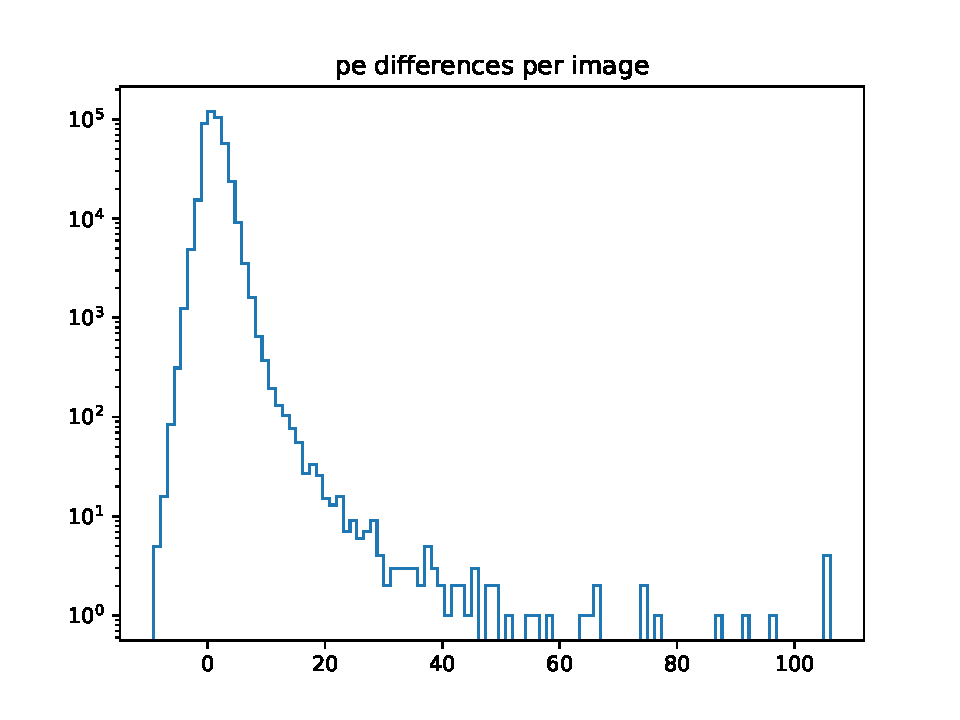
\includegraphics[width=0.5\textwidth]{Plots/diffs_hist_DBSCAN_pe_20131104_162_logy.pdf}
  }
  \subcaptionbox{Normalized distribution.\label{fig:pe_diffs}}[0.5\textwidth]{
    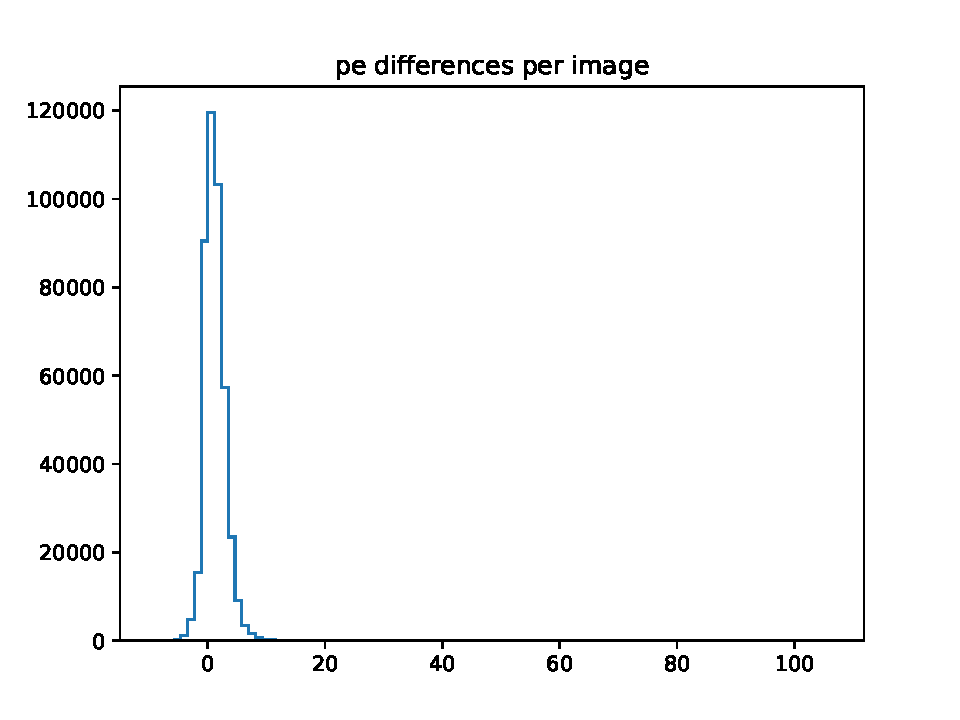
\includegraphics[width=0.5\textwidth]{Plots/diffs_hist_DBSCAN_pe_20131104_162.pdf}
  }
  \caption{PE differences per event and pixel between LP data and PhotonStream data accumulated for 300 events and normalized.}
  % \label{fig:pe_diffs}
\end{figure}
%

\autoref{fig:pe_diffs} shows the distribution of the PE differences as
described above accumulated for 300 events. The PhotonStream data on average contains
aorund 2 PE more than the corresponding LP event. However, as is visible in
\autoref{fig:pe_diffs_log} there is quite a number of pixels deviating by up to
20 PE. This reflects the observations from the four example events discussed
above: the majority of pixels contains one to two PE more than the PhotonStream
data while the few shower pixels contain a larger amount of PE more than the LP
data.


%
\begin{figure}
  \begin{subfigure}{0.5\textwidth}
    \centering
    \includegraphics[width=\textwidth, page=17]{Plots/pe_difference_pe_20131104_162.pdf}
  \end{subfigure}
  \begin{subfigure}{0.5\textwidth}
    \centering
    \includegraphics[width=\textwidth, page=26]{Plots/pe_difference_pe_20131104_162.pdf}
  \end{subfigure}
  \caption{PE differences between PhotonStream and LP data for two different events (32 and 51). The top camera image
  shows the PE as generated by the photon extractor for the PhotonStream. The
  bottom image shows the PE as generated from the LP of the time series. The
  middle image shows the difference of both images in PE per pixel.}
  \label{fig:difference}
\end{figure}
%
%
\begin{figure}
  \begin{subfigure}{0.5\textwidth}
    \centering
    \includegraphics[width=\textwidth, page=33]{Plots/pe_difference_pe_20131104_162.pdf}
  \end{subfigure}
  \begin{subfigure}{0.5\textwidth}
    \centering
    \includegraphics[width=\textwidth, page=53]{Plots/pe_difference_pe_20131104_162.pdf}
  \end{subfigure}
  \caption{PE differences between PhotonStream and LP data for two different events (67 and 111). The top camera image
  shows the PE as generated by the photon extractor for the PhotonStream. The
  bottom image shows the PE as generated from the LP of the time series. The
  middle image shows the difference of both images in PE per pixel.}
  \label{fig:difference2}
\end{figure}


%%%%%%%%%%%%%%%%%%%%%%%%%%%%%%%%%%%%%%%%%%%%%%%%%%%%%%%%%%%%%%%%%%%%%
\section{Standard Features on the PhotonStream}
%%%%%%%%%%%%%%%%%%%%%%%%%%%%%%%%%%%%%%%%%%%%%%%%%%%%%%%%%%%%%%%%%%%%%
%
Using the single extracted photons from the PhotonStream, every classical
analysis parameter can be generated, because the photons can be accumulated
along their time axis to reproduce a camera image like the one from LP data. Of
course, the big ooportunity of the PhotonStream is the additional timing
information per photon, which may yield new possibilities for analyses.
Nonetheless, it is neccessary to understand the differences on known territory
and thus to examine the classical features. For the general purpose of
parametrizing events and analysing them, an open python package called
\texttt{FeatureStream}~\cite{FeatureStream} has been developed. It contains
functions for all the data preparation steps and already contains a large
fraction of the classical features, along with some PhotonStream-specific ones.

\begin{figure}
  \begin{subfigure}{0.5\textwidth}
    \centering
  \includegraphics[width=\textwidth, page=5]{Plots/std_phs_comparison_hist_same_DBSCAN_crab.pdf}
  \end{subfigure}
  \begin{subfigure}{0.5\textwidth}
    \centering
    \includegraphics[width=\textwidth, page=5]{Plots/comparison_data_dl3.pdf}
  \end{subfigure}
  \caption{\texttt{size} of the air-shower for the same events on PhotonStream data and DBSCAN cleaning (blue) and on LP data and FACT-Tools cleaning (orange).}
  \label{fig:size_comp}
\end{figure}
%
When comparing the \texttt{size} of the same events in PhotonStream data and LP data (\autoref{fig:size_comp}),
the conclusions from \autoref{sec:ph_ex} are confirmed: As shown in
\autoref{sec:ph_ex}, the photon extraction is generally reconstructing more PE
than LP data, especially within air-shower pixels, therefore also leading to
larger air-shower clusters than the classical approach.

The main features from the Hillas parametrization are \texttt{width} and
\texttt{length} along with higher order statistical moments and the
air-shower's \texttt{size}. \autoref{fig:feat_comp} shows the Hillas features for the same events on PhotonStream data and DBSCAN cleaning (blue) and on LP data and FACT-Tools cleaning (orange).
%
\begin{figure}
  \begin{subfigure}{0.5\textwidth}
    \centering
    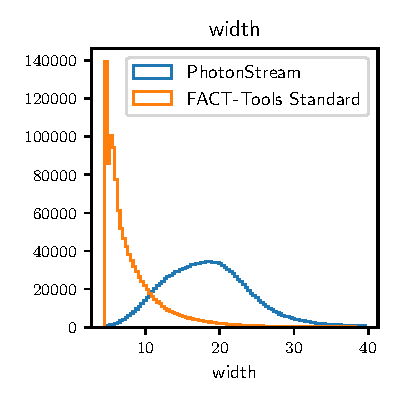
\includegraphics[width=\textwidth, page=1]{Plots/std_phs_comparison_hist_same_DBSCAN_crab.pdf}
  \end{subfigure}
  \begin{subfigure}{0.5\textwidth}
    \centering
    \includegraphics[width=\textwidth, page=2]{Plots/std_phs_comparison_hist_same_DBSCAN_crab.pdf}
  \end{subfigure}
  \begin{subfigure}{0.5\textwidth}
    \centering
    \includegraphics[width=\textwidth, page=3]{Plots/comparison_data_dl3.pdf}
  \end{subfigure}
  \begin{subfigure}{0.5\textwidth}
    \centering
    \includegraphics[width=\textwidth, page=4]{Plots/comparison_data_dl3.pdf}
  \end{subfigure}
  \caption{Hillas features for the same events on PhotonStream data and DBSCAN cleaning (blue) and on LP data and FACT-Tools cleaning (orange).}
  \label{fig:feat_comp}
\end{figure}
%
The direct comparison of the PhotonStream data's features illustrates the
differences of the cleaned air-showers: The air-shower's spatial features like
\texttt{width} and \texttt{length} are strongly shifted towards larger values.
From this it becomes clear that the DBSCAN cleaning is associating photons to
the shower cluster that lie within pixels far from the shower core, when
comparing to the classical cleaning. For the DBSCAN cleaning in the chosen
metric, photons that arrive in a close temporal proximity but within pixels not
containing large amounts of PE, can still easily be considered part of the
air-shower.

From these deviations another important question arises: how well do the MC
simulations describe the reality or in other words do simulations and data
match as expected? Without knowing which photons within an event are air-shower
photons and which not it is hard to tell, whether the different topology of the
PhotonStream clusters is closer to the real air-shower or not.
\textcolor{red}{[Untersuchungen von Sebastian?]} Independent from that it is crucial to
have that same behaviour on simulations. \autoref{fig:feat_dbscan} shows the
distributions of \texttt{width}, \texttt{length} and \texttt{size} of
PhotonStream data on the DBSCAN cleaning for data and the gamma and proton MC
simulations.

The vast majority of the observed data is generally expected to be proton
events or other background. Therefore, the distributions of data and proton MC
should be more or less similar. When comparing the distributions in
\autoref{fig:feat_dbscan} there seems to be a shift of the proton MC
simulations to slightly higher values for \texttt{width} and \texttt{length}.
So the air-shower clusters reconstructed on the proton MC simulations are
usually a bit bigger. Apart from that the distributions show a similar shape.
When comparing the \texttt{size} of the found air-showers, the data events
contain a lot more small-sized events than the simulated proton MC. This is
expected, because the data naturally contains a lot of noise and other rather
low energy events with small sizes. However, the distributions show very
similar structures on the whole range, even at the lower end. Spatially bigger
air-showers and bigger values for \texttt{size} in the MC simulations might
appear due to missing noise events in the simulations.

When expanding the DBSCAN clustering by excluding very dark pixels from the
calculations of \texttt{width} and \texttt{length},
\autoref{fig:feat_dbscan_perc}, the proton MC distributions of those features
are shifted to smaller values, as expected. The distributions of the features
on data are not really affected much, resulting in a better agreement of data
and MC simulations.
%
\begin{figure}
  \begin{subfigure}{0.5\textwidth}
    \centering
    \includegraphics[width=\textwidth, page=23]{Plots/data_mc/features_DBSCAN.pdf}
  \end{subfigure}
  \begin{subfigure}{0.5\textwidth}
    \centering
    \includegraphics[width=\textwidth, page=13]{Plots/data_mc/features_DBSCAN.pdf}
  \end{subfigure}
  \begin{subfigure}{0.5\textwidth}
    \centering
    \includegraphics[width=\textwidth, page=15]{Plots/data_mc/features_DBSCAN.pdf}
  \end{subfigure}
  \begin{subfigure}{0.5\textwidth}
    \centering
    \includegraphics[width=\textwidth, page=8]{Plots/data_mc/features_DBSCAN.pdf}
  \end{subfigure}
  \caption{Features of the reconstructed air-showers using the DBSCAN cleaning. The blue histograms show the observed data, whereas orange and green show proton and gamma MC simulations respectively.}
  \label{fig:feat_dbscan}
\end{figure}
%
%
\begin{figure}
  \begin{subfigure}{0.5\textwidth}
    \includegraphics[width=\textwidth, page=23]{Plots/data_mc/features_DBSCAN_perc.pdf}
  \end{subfigure}
  \begin{subfigure}{0.5\textwidth}
    \includegraphics[width=\textwidth, page=13]{Plots/data_mc/features_DBSCAN_perc.pdf}
  \end{subfigure}
  \caption{Features of the reconstructed air-showers using DBSCAN and additionally excluding pixels with less than $\SI{1}{\percent}$ PE of the air-shower's total \texttt{size}. The blue histograms show the observed data, whereas orange and green show proton and gamma MC simulations respectively.}
  \label{fig:feat_dbscan_perc}
\end{figure}
%
From the feature distributions it becomes clear that there are regions, where
data and MC simulations fit better. The \texttt{size} is in better agreement
above a threshold of about \num{100}. In general, events with a big size are
less prone to reconstruction errors, since  noise fluctuations in the number of
PE and in the spatial distribution of photons, both affecting the origin
reconstruction, are suppressed. Small clusters, especially within the data
might very well also be noise events. However, they appear in data, but are not
accounted for in the MC simulations used for training the random forests, making them a likely source of error.

Especially with respect to the origin reconstruction, the number of pixels
\texttt{n\_pixel} associated with an air-shower is important for the accuracy
of the reconstructed position. Very small events are strongly influenced by
fluctuating neighboring pixels and the main axis direction is generally hard to
reconstruct. Due to the quantization of the single pixels a singular photon
within a neighboring pixel can impact the result significantly.
The optimization of the cuts on all used features has to be performed in
detail beyond the scope of this thesis, but to investigate the potential of the
PhotonStream data, the quality cuts are restrained to those excluding events,
which are intrinsically prone to reconstruction errors.

%%%%%%%%%%%%%%%%%%%%%%%%%%%%%%%%%%%%%%%%%%%%%%%%%%%%%%%%%%%%%%%%%%%%%
\section{Time Features on the PhotonStream}
%%%%%%%%%%%%%%%%%%%%%%%%%%%%%%%%%%%%%%%%%%%%%%%%%%%%%%%%%%%%%%%%%%%%%
%
The PhotonStream does not only open the possibilities for analyses of single
photon features, while still containing all relevant data from the classical
representation, it furthermore contains \textbf{time information} per photon.
This additional dimension in the data makes it even more interesting for
analyses and might promise great advances in performance.

With the additional time information a series of new features can be
implemented. The classical features can be expanded onto this dimension,
examining the light distributions along the time axis and calculating
statistical moments of them. There are additional angles describing the
shower's position when working in three dimensions, and new features can be
engineered. These new features possibly offer a way to strongly boost
performance by taking advantage of the new additional dimension.

The distributions of arrival times of the single photons for data and MC
simulations are shown in \autoref{fig:slices}. The histograms show the arrival
times for every single photon of 2000 events normalized to an area of 1. The
top histogram represents all arriving photons. It becomes clear that there
seems to be a significant discrepancy between the MC simulations and data.
While distributions of the MC simulations of both, gammas and protons, quite
resemble each other, the data distribution shows a very different picture. The
most common arrival time of data lies way beyond the one on MC simulations.
Furthermore, the structure of the distribution before the main peak in data
shows two dips and generally not a very clear distribution as compared to the
monotonous rise of the MC distributions. This behaviour might result from noise
events and falsely triggered events or originate from electronic artifacts. To
investigate the origins of this structure, the bottom histogram shows the
arrival times of all photons located in pixels with at least \num{10} photons.
This way the fraction of non air-shower photons becomes very small. In the
result the normally distributed underground, as seen in the top histogram,
vanishes almost completely. The most common arrival times for the MC
simulations become sharper but remain at the same position as before. In
contrast to the complete events, the data distribution now shows a peak near to
the ones in the MC simulations and does no longer show the unstructered
behaviour in the first \num{40} time slices as described above. The difference
between data and MC simulations still manifests between time slices \num{60}
and \num{80}, though. The data distribution decreases slower and takes about
\num{20} time slices more to return to a supposed background level.
%
\begin{figure}
  \begin{subfigure}{\textwidth}
    \centering
    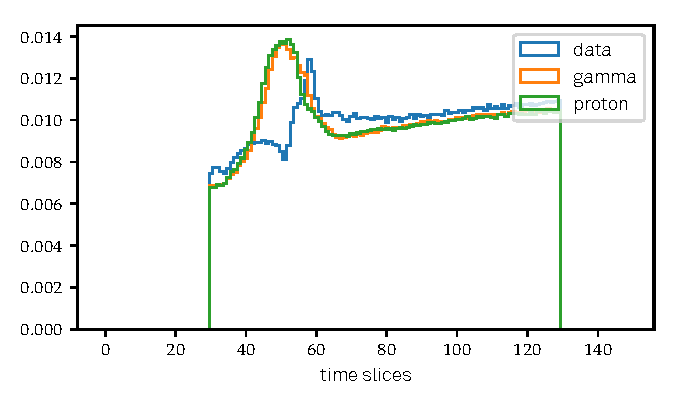
\includegraphics[width=0.8\textwidth]{Plots/all_slices_min_0_per_pixel.pdf}
  \end{subfigure}
  \begin{subfigure}{\textwidth}
    \centering
    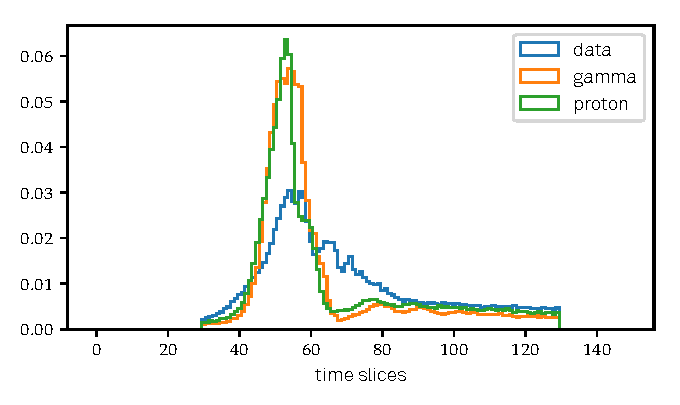
\includegraphics[width=0.8\textwidth]{Plots/all_slices_min_10_per_pixel.pdf}
  \end{subfigure}
  \caption{Arrival times of the single photons within all the pixels (top) and the cleaned air-shower pixels containing at least 10 photons (bottom) on data and MC simulations.}
  \label{fig:slices}
\end{figure}
%

The arrival time distributions show quite some disagreement in uncleaned
pixels, originating from data-MC-mismatches probably due to noise effects. For
the cleaned images, which are the crucial ones, the agreement is better, so
implementing time features into a working PhotonStream analysis is a natural
next step.

%%%%%%%%%%%%%%%%%%%%%%%%%%%%%%%%%%%%%%%%%%%%%%%%%%%%%%%%%%%%%%%%%%%%%
\section{Reconstruction of the Source Position}
%%%%%%%%%%%%%%%%%%%%%%%%%%%%%%%%%%%%%%%%%%%%%%%%%%%%%%%%%%%%%%%%%%%%%
%
As described in \autoref{sec:source_pos} the reconstruction of the source
position uses the air-shower's features \texttt{delta}, \texttt{width} and
\texttt{length}. The calculated angle \texttt{delta} plays a major role in
finding the right source position, since it describes the axis along which
the source position is assumed to be. It is calculated as the angle between
the shower's main axis and the camera's $x$-axis. Therefore, it is dependant
on the covariance of the light distribution and thus affected by the
differences within the PhotonStream.

To investigate the differences on PhotonStream data, it is possible to
calculate a true delta on the data images by using the telescope's pointing
position. From the pointing position and the known source position an
expected source position within the camera can be calculated. The
air-shower's cog and the calculated source position within the camera can
then be used to calculate a vector representing the estimated shower axis.
The calculated angle $\delta_\text{true}$ of that shower axis can thus be
compared to the calculated angle of the cleaned air-shower's main axis. The
distribution of these differences is expected to have two peaks: one around
zero and one around a difference of $\pi$. These two peaks correspond to
air-showers with a very small difference in $\delta$ and on the one hand the
right estimated sign of \texttt{disp} (zero) and on the other hand the
opposite estimated sign of \texttt{disp} ($\pi$). When dividing the
distribution into the different signs of \texttt{disp} there should only be
one peak for each distribution for a working sign classifier.

\autoref{fig:delta_fact} shows a distribution of $\symup{\Delta}\delta$ for
the pixel based cleaning as described in \autoref{sec:thresh} on LP data.
The two histograms represent the different estimations of the sign of
\texttt{disp} for the whole open data sample. The distributions show very
good agreement with the expectations described above. While this is not a
comparison with any real truth, it nevertheless shows a working
reconstruction of the air-shower events.
%
\begin{figure}
  \centering
  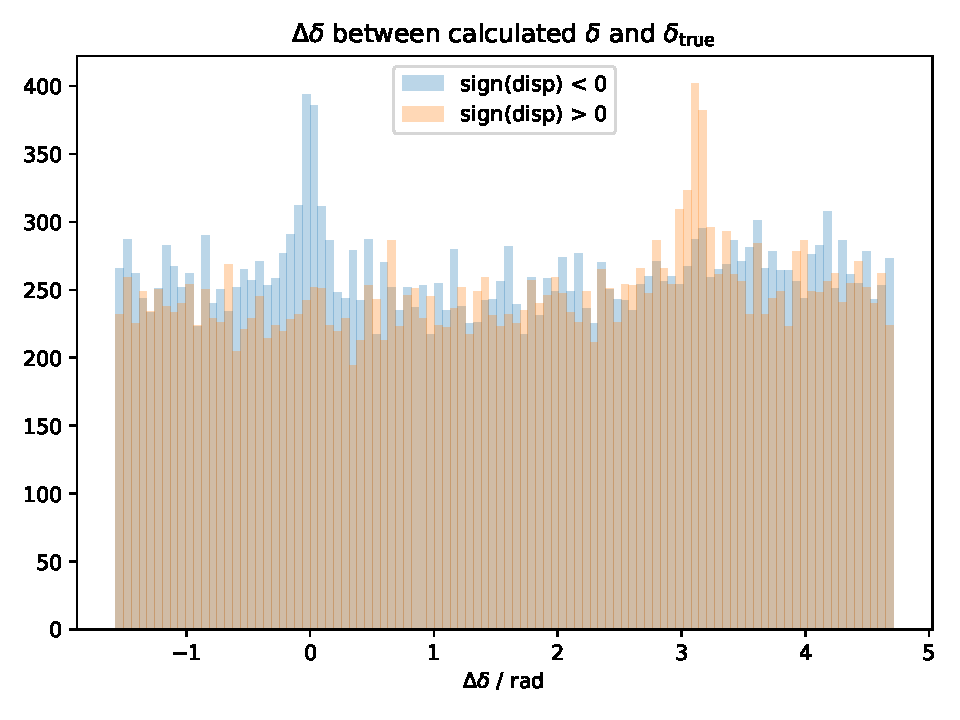
\includegraphics[width=0.7\textwidth]{Plots/delta_delta/delta_delta_facttools.pdf}
  \caption{Difference between calculated delta and true delta for the FACT-Tools analysis \cite{openana}. The distributions show the calculated $\symup{\Delta}\delta$ for the different predictions of sign of \texttt{disp} on the whole open data crab sample.}
  \label{fig:delta_fact}
\end{figure}
%
When calculating $\symup{\Delta}\delta$ on the cleaned PhotonStream data, a
very different picture emerges. \autoref{fig:delta_diff_a} shows
$\symup{\Delta}\delta$ for the DBSCAN cleaning, when projecting the found
photons back to the camera plane and calculating \texttt{delta}. There are
hardly any peaks in these distributions, but rather widely spread
accumulation ranges around zero and $\pi$. Thus, the calculated
\texttt{delta} seems to differ quite sicnificantly from the expected
\texttt{delta}. Furthermore, both \texttt{sign} predictions show similar
distributions, hinting at a low accuracy for the \texttt{sign}
classification. The main differrence between the air-showers found by DBSCAN
and the ones found by the classic cleaning projected to the camera plane is
the spread across the camera axes. DBSCAN clustering is associating photons
from pixels quite distant from the shower core to the air-shower cluster.
This way, the spread within $x$ and $y$ becomes way bigger. Because
\texttt{delta} is calculated on the $x$-$y$-distribution weighted by the
number of photons, these outlier photons might have a big impact on the
calculation of \texttt{delta}, even though they usually only contain very
few photons. To prevent this from happening, the cleaning can be extended by
a step excluding pixels with less than $\SI{1}{\percent}$ of the total
amount of photons from the calculations of \texttt{delta}, \texttt{length}
and \texttt{width}. The distributions of $\symup{\Delta}\delta$ for this
cleaning are shown in \autoref{fig:delta_diff_perc}.

\begin{figure}
  \subcaptionbox{\label{fig:delta_diff_a}}[0.48\textwidth]{
    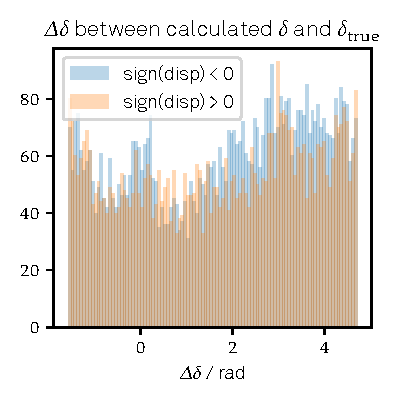
\includegraphics[width=0.5\textwidth]{Plots/delta_delta/delta_true_diff_hist_thresholds_rad_20131104_162.pdf}
  }
  \subcaptionbox{\label{fig:delta_diff_perc}}[0.48\textwidth]{
    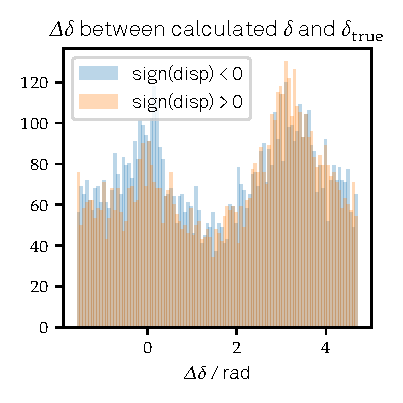
\includegraphics[width=0.5\textwidth]{Plots/delta_delta/delta_delta _DBSCAN_1perc_rad_20131104_162.pdf}
  }
  \caption{Difference between calculated delta and true delta for a subset of 500 data events. delta is calculated using all cleaned pixels \protect\subref{fig:delta_diff_a} and using only cleaned pixels containing more than $\SI{1}{\percent}$ of the air-shower's size \protect\subref{fig:delta_diff_perc}.}
  \label{fig:true_delta}
\end{figure}
%
The distributions change significantly, when adapting the cleaning.
The two peaks become quite distinctive around $0$ and $\pi$. Also the
different sign predictions show different heights around the two
accumulation points corresponding to the rightly classified signs, although
there seem to be frequent misclassifications. Although the results still
differ strongly from the ones shown in \autoref{fig:delta_fact}, the
accuracy of delta improves when neglecting outlying pixels. Thus, there
seems to be an impact of the large spread of DBSCAN clusters which is very
likely to also affect the origin reconstruction on such events.

%
\begin{figure}
  \centering
  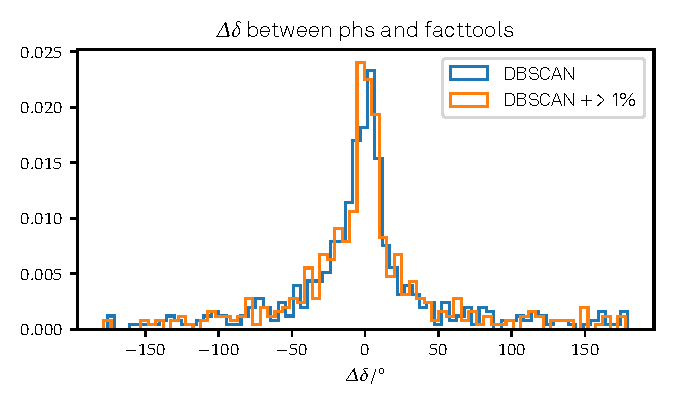
\includegraphics[width=\textwidth]{Plots/delta_delta/delta_diff_hist_perc_and_normal_DBSCAN_delta_20131104_162.pdf}
  \caption{Differences between the PhotonStream \texttt{delta} and the FACT-Tools \texttt{delta} for the DBSCAN cleaning (blue) and the DBSCAN cleaning extended by excluding pixels with less than $\SI{1}{\percent}$ of the shower's \texttt{size} (orange).}
  \label{fig:delta}
\end{figure}
%
Since the FACT-Tools analysis yields good results and a working origin
reconstruction, the differences between its features and the DBSCAN cluster
features can also be investigated to understand the new data representation.
\autoref{fig:delta} shows the differences between the PhotonStream
\texttt{delta} and the FACT-Tools \texttt{delta} for the DBSCAN cleaning (blue
histogram) and the DBSCAN cleaning extended by excluding pixels with less
than $\SI{1}{\percent}$ of the shower's \texttt{size} (orange histogram).
From these distributions, it becomes clear that the difference of the
PhotonStream's air-showers does not solely result from the wider spread of
the light distribution over the camera pixels. The two distributions barely
differ from another, although as shown by \autoref{fig:delta_diff_perc}, the
reconstruction of \texttt{delta} seems to improve with the additional
cleaning. For the majority of events the calculated \texttt{delta} is within
$\mathcal{O}(\SI{10}{\degree})$ to the FACT-Tools \texttt{delta}, but for the
origin reconstruction such a difference can become a difficult obstacle.
However, this comparison, as the one with the expected source position
within the camera, is not a comparison with truth values, but rather one
with a working analysis.

%%%%%%%%%%%%%%%%%%%%%%%%%%%%%%%%%%%%%%%%%%%%%%%%%%%%%%%%%%%%%%%%%%%%%
\subsection{Reconstruction of the Source Position on Data}
%%%%%%%%%%%%%%%%%%%%%%%%%%%%%%%%%%%%%%%%%%%%%%%%%%%%%%%%%%%%%%%%%%%%%

All these investigations, of course, serve the sole purpose of understanding
the different prerequisites for reconstructing the source position on
air-shower images. As described in \autoref{sec:source_pos} this is done by
using the \texttt{disp} method on Hillas parametrized images. Random forests
are used to estimate $|\texttt{disp}|$ via a regression task and then determine
the $\text{sign}(\texttt{disp})$ via a classification. The used random forests
consist of \num{100} estimators, each of which has a maximum depth of \num{15}.

The output of these random forests can then be projected from the air-shower's
core within the camera to sky coordinates, resembling the estimated source
position. Since the Crab Nebula is a well known source with a well known
position, the difference between the reconstructed and the knwon source
position can be calculated. It is tipically quantized as the euklidian distance
squared in $[\theta^2] = \si{\degree\squared}$ and illustrated as shown in
\autoref{fig:theta2}. These $\theta^2$-plots show the distribution of the
distances squared of the reconstructed source position per event from the Crab
Nebula's known position. They contain all events after preselection cuts and
applying the gamma hadron separation at a specific \texttt{gamma\_prediction}
threshold. The blue bins show the reconstructed signal events (On events) when
pointing directly to the source position while the orange bins represent the
reconstructed background events (Off events), pointing to the night sky next to
the source. The $\theta^2$-cut, represented by the dashed, grey vertical line,
represents the optimal cut for the source's signal events. Events between
\num{0} and this cut are considered when calculating the excess significance.
The ratio of on-source observation time and off-source observation time is
\num{0.2}. This fraction is used to estimate the background within the
on-source observations. Both, $\theta^2$-cut and the \texttt{gamma\_prediction}
threshold are determined by finding the highest significance, calculated as
described by Li \& Ma \cite{LiMa}.

The used random forest is trained on gamma and proton MC simulations to perform
the \texttt{disp} regression and the \texttt{sign} classification. The
performance results of this training are very good for the \texttt{sign}
classification, while the regression of \texttt{disp} seems to be more
difficult. The accuracy of the \texttt{sign} classification averaged from the
cross-validation is $0.7923\,\pm\,0.0018$. Slightly outperforming the FACT-
Tools analysis with an accuracy of $0.7537\,\pm\,0.0018$. The regression of
\texttt{disp}, however, only reaches an $R^2$ score of $0.5385\,\pm\,0.0046$,
which is quite low and might strongly affect the accuracy of the origin
reconstruction. The FACT-Tools analysis, in comparison, reaches an $R^2$ score
of $0.6631\,\pm\,0.0044$.

For a Crab Nebula data sample and a working analysis the $\theta^2$-plot is
expected to have an equally distributed, low number of Off-events with a
significant excess of On-events as close to $\theta^2 = 0$ as possible. From
the results shown in \autoref{fig:theta2} it becomes very clear, that the
reconstruction of the PhotonStream data in the way described above does not
yield a very good source reconstruction on data. The optimal $\theta^2$-cuts
around \num{0.1} are quite large. The distribution of the On-events around the
true source position are rather fuzzy: there is no clear peak, especially not
around \num{0}. The source excess starts around \num{0.10} and grows until
between \num{0} and \num{0.05}. Thus, the reconstruction of the source position
and especially the regression of \texttt{disp} seem to have a big error margin,
reconstructing events to the close proximity of the true source position. Since
$\theta$ is not the error on the reconstructed position, but rather the
distance of all cleaned events to a specific source, the cleaning and
especially the gamma hadron separation affect the results.
%
\begin{figure}
  \begin{subfigure}{\textwidth}
    \centering
    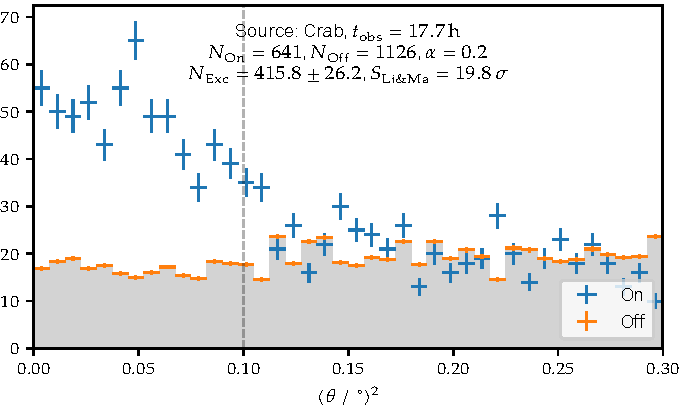
\includegraphics[width=\textwidth]{Plots/results/DBSCAN/theta2_plot.pdf}
  \end{subfigure}
  \begin{subfigure}{\textwidth}
    \centering
    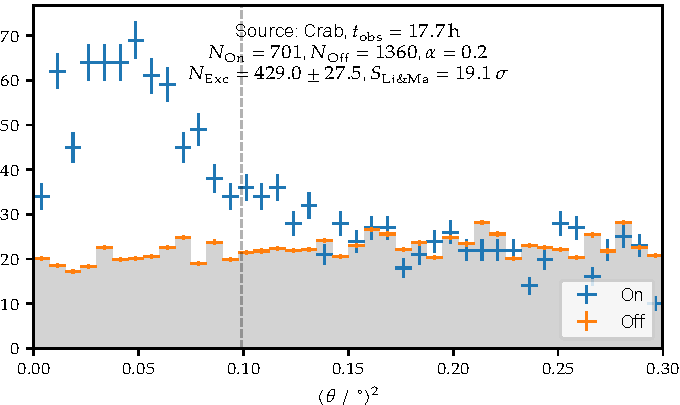
\includegraphics[width=\textwidth]{Plots/results/DBSCAN_perc/theta2_plot.pdf}
  \end{subfigure}
  \caption{$\theta^2$-plots for the PhotonStream data and dedicated analysis for the DBSCAN cleaning (top) and extended by excluding pixels with less than $\SI{1}{\percent}$ of the air-shower's \texttt{size} (bottom). They contain all events after preselection cuts and applying the gamma hadron separation at a specific \texttt{gamma\_prediction} threshold. The blue bins show the reconstructed signal events (On events) when pointing directly to the source position while the orange bins represent the reconstructed background events (Off events), pointing to the night sky next to the source.}
  \label{fig:theta2}
\end{figure}
%

%%%%%%%%%%%%%%%%%%%%%%%%%%%%%%%%%%%%%%%%%%%%%%%%%%%%%%%%%%%%%%%%%%%%%
\section{Gamma Hadron Separation}
%%%%%%%%%%%%%%%%%%%%%%%%%%%%%%%%%%%%%%%%%%%%%%%%%%%%%%%%%%%%%%%%%%%%%
%
The observed data mainly consists of proton events, since the majority of the
cosmic ray flux consists of protons. Therefore, it is important to distinguish
gamma air-shower events from proton events, which are considered background for
this analysis. A working gamma hadron separation affects all steps of the
analysis, because the energy reconstruction is trained on gamma events as well
as the source reconstruction. A badly cleaned data set thus will not work well
with the trained models.

For this analysis a random forest is used for the classification. It consists
of \num{100} decision trees and a maximum depth of \num{15} for the single
tree. The forest is trained on the features shown in \autoref{fig:sep_feat}.
This figure also shows the proportional importances of the single features
within the trained model. The most important features for the separation are
the \texttt{width} and \texttt{kurtosis\_trans}, the higher order statistical
moment along the same axis. From this, one can see that the spatial topology of
the air-shower is the main discriminator.

% neccessary line ^^^^
\begin{figure}
  \centering
  \includegraphics[width=0.8\textwidth, page=4]{Plots/results/DBSCAN/separation_performance.pdf}
  \caption{Features used for the gamma hadron separation model. The features are defined in \autoref{sec:params} and sorted by their importance for the separation task.}
  \label{fig:sep_feat}
\end{figure}
%
The trained model can be validated on the MC data, because the particle type is
known for the datasets. To do so, the model is trained on a subset of the
available simulations to then be validated on the small contemplementary
dataset. To avoid statistical fluctuations within the subsamples to affect the
results, a cross-validation is used. \autoref{fig:sep_auc} shows the ROC curve
of the trained model, consisting of the true positive rate dependant on the
false positive rate. The blue line shows the results of the averaging from the
cross-validation. The AUC is $0.8425\,\pm\,0.0016$ with the error resulting
from the averaging. This is a very good result for the separation of the gamma
showers from the proton background, especially since this analysis is not
primarily focused on optimizing these metrics. However, this is a result on
Monte Carlo simulations and the quality of the model on data might differ quite
significantly.
%
\begin{figure}
  \centering
  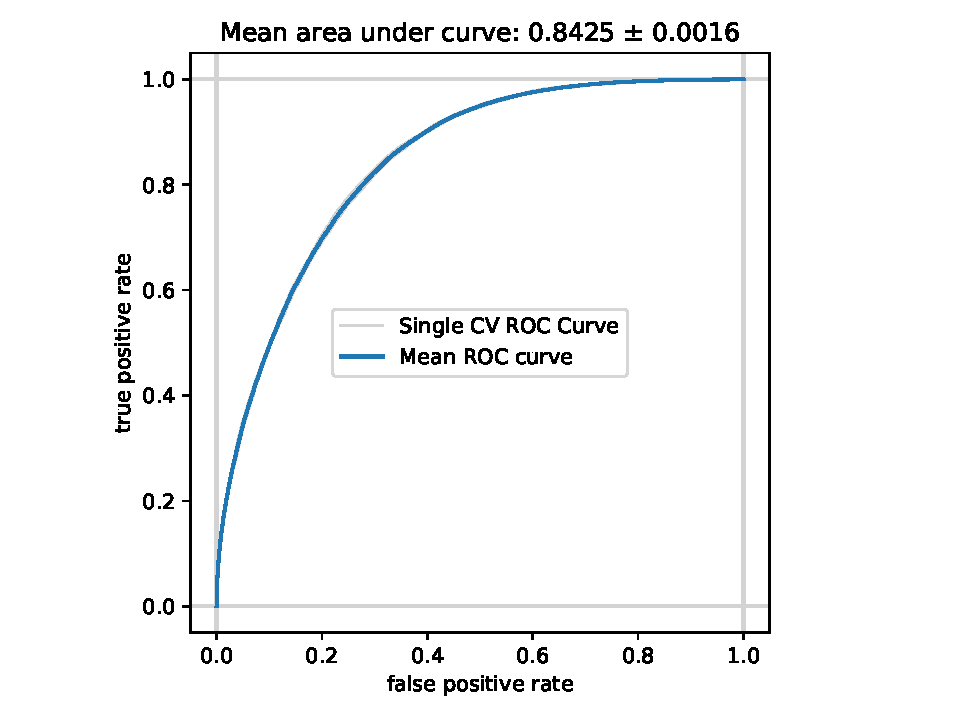
\includegraphics[width=0.8\textwidth, page=1]{Plots/results/DBSCAN/separation_performance.pdf}
  \caption{\textit{Receiver Operating Characteristic} (ROC) curve for the binary gamma hadron separation. The true positive rate dependant on the false positive rate is shown in grey. The blue line represents the averaged result out of a 5-fold cross-validation. The averaged \textit{area under curve} (AUC) from the 5-fold cross-validation for the trained models is $0.8425\,\pm\,0.0016$ with the error resulting from the averaging.}
  \label{fig:sep_auc}
\end{figure}
%
%
% \begin{figure}
%   \centering
%   \includegraphics[width=0.8\textwidth, page=3]{Plots/results/DBSCAN/separation_performance.pdf}
%   \caption{Gamma hadron separation plot.}
%   \label{fig:sep2}
% \end{figure}
%
%%%%%%%%%%%%%%%%%%%%%%%%%%%%%%%%%%%%%%%%%%%%%%%%%%%%%%%%%%%%%%%%%%%%%
\section{Energy Estimation}
%%%%%%%%%%%%%%%%%%%%%%%%%%%%%%%%%%%%%%%%%%%%%%%%%%%%%%%%%%%%%%%%%%%%%
%
The reconstruction of the air-shower's energy is applied on cleaned and as
gamma air-shower classified images. It uses the same features as the separation
model. Since the PhotonStream paired with DBSCAN reconstructs bigger air-shower
images and a larger number of photons it is interesting to investigate the
results on the reconstructed energy.

For this analysis a random forest is used for the energy estimation, as well.
It performs a regression task and consists of \num{100} decision trees and a
maximum depth of \num{15} for the single tree. The forest is trained on the
features shown in \autoref{fig:energy_feat}. In addition to the features described in \autoref{sec:params}, the \texttt{area} of the shower is used for the energy estimation. It is defined as
%
\begin{equation}
  \texttt{area} = \texttt{width}\times\texttt{length}\times\symup{\pi}\, .
\end{equation}
%
\autoref{fig:energy_feat} also shows the
proportional importances of the single features within the trained model. The
most important features for the energy estimation of a shower are those
strongly correlated with the number of photons within the air-shower. The
\texttt{size} and the number of pixels associated with the air-shower
(\texttt{n\_pixel}) are by far the most important features, together making up
almost $\sfrac{2}{3}$ of the total importance. Of course, since the number of
photons depends on the number and energy of secondary particles, which itself
depends on the energy of the primary particle, one would expect that.
%
\begin{figure}
  \centering
  \includegraphics[width=0.9\textwidth, page=4]{Plots/results/DBSCAN/energy_performance.pdf}
  \caption{Features used for the energy estimation model. The features are defined in \autoref{sec:params} and sorted by their importance for the estimation task.}
  \label{fig:energy_feat}
\end{figure}
%

Since the primary particle's energy an air-shower was simulated with is known
for the simulation data, the performance of the trained model can be
validated on the MC simulations. \autoref{fig:energy_matr} shows the confusion
matrix for the energy estimation. The energy estimated by the random forest
($y$-axis) is shown against the event's true energy ($x$-axis). A clear
correlation is visible on the diagonal, showing that the trained model is
reconstructing energies close to the true energies. Rather than a thin line,
the spread of this distribution however is quite wide. The reconstructed
energies therefore lie within a wide error margin around the true energy.
Especially for low energies the spread becomes very large. Air-showers
resulting from low energy primary particles contain less Cherenkov photons, as
described above. Therefore the reconstructed air-shower not only contains less
photons but also illuminates a smaller area of the camera. Thus, fluctuations
become more important and the accurate reconstruction of the image features more
difficult. Low energy events consequently are intrinsically harder to assign
the right energy to.
%
\begin{figure}
  \centering
  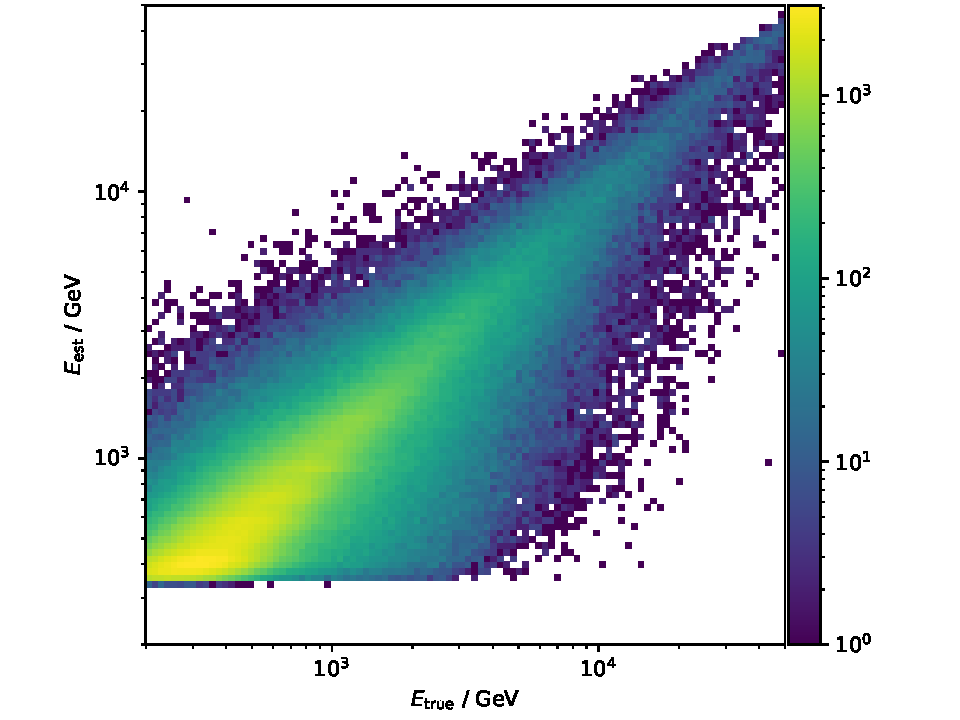
\includegraphics[width=0.9\textwidth]{Plots/results/DBSCAN/energy_migration.pdf}
  \caption{Confusion matrix for the estimation of the primary particle's energy. The energy estimated by the random forest ($y$-axis) is shown against the event's true energy ($x$-axis).}
  \label{fig:energy_matr}
\end{figure}
%
The resulting $R^2$ score for the best energy estimation model on PhotonStream
data is $R^2 = 0.74$. This is a quite good score for the energy estimation and
shows that the energy reconstruction works well on the gamma MC simulations.
Especially when compared to the FACT-Tools open data analysis~\cite{openana},
which reaches an $R^2$ score of $0.6876$, this result outperforms the
classical analysis.
%
% The energy bias and resolution of the analysis are shown for bins of true gamma
% energy in \autoref{fig:bias}.
% %
% \begin{figure}
%   \centering
%   \includegraphics[width=0.9\textwidth]{Plots/results/DBSCAN/bias_resolution.pdf}
%   \caption{Bias (blue histogram) and resolution (orange histogram) of the PhotonStream data on DBSCAN cleaning as a function of true Energy of the gamma rays.}
%   \label{fig:bias}
% \end{figure}
% %


%%%%%%%%%%%%%%%%%%%%%%%%%%%%%%%%%%%%%%%%%%%%%%%%%%%%%%%%%%%%%%%%%%%%%
\section{Parameters of DBSCAN}
%%%%%%%%%%%%%%%%%%%%%%%%%%%%%%%%%%%%%%%%%%%%%%%%%%%%%%%%%%%%%%%%%%%%%
%
The physical properties used for this analysis are derived from the cleaned
images, i.e. the reconstructed shower clusters. The reconstruction of these
clusters is done by the DBSCAN algorithm. To set the right topology for the
clustering, DBSCAN is defined by two dedicated parameters, as described in
\autoref{sec:phs_clean}. The used parameters can be optimized for the analysis,
as well. However, there does not appear to be reason to believe that an
analysis specific set of the two parameters needs to be derived.

The minimum number of photons within a cluster $m$ has not been investigated. A
minimum number of \num{20} photons excludes only very small noise clusters. For
the analysis, the cuts in \texttt{size} and \texttt{n\_cluster} will then
exclude the small events.

The minimum distance $\varepsilon$ for a photon to still be associated with a
dense cluster has been investigated to be \num{0.1} for optimal results. The
effects of this parameter on the features of the air-shower clusters can be
examined nonetheless. \autoref{fig:eps_feat1}, \ref{fig:eps_feat2} and
\ref{fig:eps_feat3} show the distributions of the number of reconstructed
clusters and the spatial dimension of the air-shower represented by the
\texttt{width} for clusterings with different $\varepsilon$-configurations. To
give a picture of the dependance $\varepsilon$ is varied below and above the
default value of \num{0.1}. To simultaneously give a hint on the agreement of
MC simulations and the observed data, the proton MC simulated data (orange) is
also shown. The distributions are normalized to their observation time and the
expected night sky flux.

The effect of $\varepsilon$ on the topology of the clusters becomes very clear
when comparing the feature distributions for different values of $\varepsilon$.
The bigger $\varepsilon$ is set, the bigger the \texttt{width} gets. Therefore,
going to smaller values, the air-shower clusters will be confined to a smaller
space. The number of reconstructed clusters also gradually rises when setting
a bigger $\varepsilon$. This is to be expected, since a bigger $\varepsilon$
allows for less dense regions of the point cloud to be considered a dense
cluster. At some point this will lead to noise or ambient light to be
classified as air-shower clusters. For $\varepsilon = 0.11 / 0.12$ however, it
definiteley leads to large mismatches between MC simulations and data, that
become very clear for $\varepsilon = 0.14$. For $\varepsilon = 0.175$ the
distance for photons within a cluster becomes so big, that the initial large
number of small clusters decreases again, because many of these are combined to
a few bigger clusters.

For the observed data another development for bigger values of $\varepsilon$
emerges: The number of found air-showers within data events compared to those
found in proton MC simulations rises. This supposedly is the result of the
clustering reconstructing noise events within the data, that are not present in
the proton MC simulations. All in all, the agreement of simulations and data
seem to be best for smaller $\varepsilon$, rather than ones above \num{0.1}.

%
\begin{figure}
  \begin{subfigure}{0.5\textwidth}
    \centering
    $\symbf{\varepsilon = 0.07}$\par\smallskip
    \includegraphics[width=0.9\textwidth, page=23]{Plots/Epsilon/07_comparison.pdf}
  \end{subfigure}
  \begin{subfigure}{0.5\textwidth}
    \centering
    $\symbf{\varepsilon = 0.07}$\par\smallskip
    \includegraphics[width=0.9\textwidth, page=2]{Plots/Epsilon/07_comparison.pdf}
  \end{subfigure}
%%%%%%%%%%%%%%%%%%%%%%%%%%%%%%%%%%%%%%%%%%%%%%%%%%%%
  \begin{subfigure}{0.5\textwidth}
    \centering
    $\symbf{\varepsilon = 0.09}$\par\smallskip
    \includegraphics[width=0.9\textwidth, page=23]{Plots/Epsilon/09_comparison.pdf}
  \end{subfigure}
  \begin{subfigure}{0.5\textwidth}
    \centering
    $\symbf{\varepsilon = 0.09}$\par\smallskip
    \includegraphics[width=0.9\textwidth, page=2]{Plots/Epsilon/09_comparison.pdf}
  \end{subfigure}
  %%%%%%%%%%%%%%%%%%%%%%%%%%%%%%%%%%%%%%%%%%%%%%%%%%%%
  \caption{Distributions of the number of reconstructed
  clusters and the spatial dimension of the air-shower represented by the
  \texttt{width} for clusterings with different $\varepsilon$-configurations. To simultaneously give a hint on the agreement of MC simulations and the observed data, the proton MC simulated data (orange) is also shown. The distributions are normalized to their observation time and the expected night sky flux. The default value is $\varepsilon = 0.1$.}
  \label{fig:eps_feat1}
\end{figure}
%
%
\begin{figure}
  \begin{subfigure}{0.5\textwidth}
    \centering
    $\symbf{\varepsilon = 0.10}$\par\smallskip
    \includegraphics[width=0.9\textwidth, page=23]{Plots/Epsilon/10_comparison.pdf}
  \end{subfigure}
  \begin{subfigure}{0.5\textwidth}
    \centering
    $\symbf{\varepsilon = 0.10}$\par\smallskip
    \includegraphics[width=0.9\textwidth, page=2]{Plots/Epsilon/11_comparison.pdf}
  \end{subfigure}
  %%%%%%%%%%%%%%%%%%%%%%%%%%%%%%%%%%%%%%%%%%%%%%%%%%%%
  \begin{subfigure}{0.5\textwidth}
    \centering
    $\symbf{\varepsilon = 0.12}$\par\smallskip
    \includegraphics[width=0.9\textwidth, page=23]{Plots/Epsilon/12_comparison.pdf}
  \end{subfigure}
  \begin{subfigure}{0.5\textwidth}
    \centering
    $\symbf{\varepsilon = 0.12}$\par\smallskip
    \includegraphics[width=0.9\textwidth, page=2]{Plots/Epsilon/12_comparison.pdf}
  \end{subfigure}
  %%%%%%%%%%%%%%%%%%%%%%%%%%%%%%%%%%%%%%%%%%%%%%%%%%%%
  \caption{Distributions of the number of reconstructed
  clusters and the spatial dimension of the air-shower represented by the
  \texttt{width} for clusterings with different $\varepsilon$-configurations. To simultaneously give a hint on the agreement of MC simulations and the observed data, the proton MC simulated data (orange) is also shown. The distributions are normalized to their observation time and the expected night sky flux. The default value is $\varepsilon = 0.1$.}
  \label{fig:eps_feat2}
\end{figure}
%
%
\begin{figure}
  \begin{subfigure}{0.5\textwidth}
    \centering
    $\symbf{\varepsilon = 0.14}$\par\smallskip
    \includegraphics[width=0.9\textwidth, page=23]{Plots/Epsilon/14_comparison.pdf}
  \end{subfigure}
  \begin{subfigure}{0.5\textwidth}
    \centering
    $\symbf{\varepsilon = 0.14}$\par\smallskip
    \includegraphics[width=0.9\textwidth, page=2]{Plots/Epsilon/14_comparison.pdf}
  \end{subfigure}
  %%%%%%%%%%%%%%%%%%%%%%%%%%%%%%%%%%%%%%%%%%%%%%%%%%%%
  \begin{subfigure}{0.5\textwidth}
    \centering
    $\symbf{\varepsilon = 0.175}$\par\smallskip
    \includegraphics[width=0.9\textwidth, page=22]{Plots/Epsilon/175_comparison.pdf}
  \end{subfigure}
  \begin{subfigure}{0.5\textwidth}
    \centering
    $\symbf{\varepsilon = 0.175}$\par\smallskip
    \includegraphics[width=0.9\textwidth, page=2]{Plots/Epsilon/175_comparison.pdf}
  \end{subfigure}
  %%%%%%%%%%%%%%%%%%%%%%%%%%%%%%%%%%%%%%%%%%%%%%%%%%%%
  \caption{Distributions of the number of reconstructed
  clusters and the spatial dimension of the air-shower represented by the
  \texttt{width} for clusterings with different $\varepsilon$-configurations. To simultaneously give a hint on the agreement of MC simulations and the observed data, the proton MC simulated data (orange) is also shown. The distributions are normalized to their observation time and the expected night sky flux. The default value is $\varepsilon = 0.1$.}
  \label{fig:eps_feat3}
\end{figure}
%
To investigate the effects of $\varepsilon$ further on a higher level than the
feature distributions, the scores used to validate the analysis results can be
investigated in dependancy to the value of $\varepsilon$. To do so, these
scores are shown in \autoref{fig:eps_scores}, \ref{fig:eps_sigma} and
\ref{fig:eps_theta} for $\varepsilon \in [0.07,\,0.1]$. \autoref{fig:eps_sigma}
additionally contains smaller values of $\varepsilon$. No real dependancy can
be seen and the results seem to be the same throughout the variation. Except
for the number of reconstructed air-showers, which decreases strongly for small
$\varepsilon$, resulting in the sharply decreasing detection significance in
\autoref{fig:eps_sigma}.
%
\begin{figure}
  \centering
  \includegraphics[width=0.85\textwidth]{Plots/Epsilon/eps_scores.pdf}
  \caption{Validation scores for the analysis tasks in dependance of the DBSCAN's $\varepsilon$. The AUC for the gamma hadron separation's ROC (blue), the source position reconstruction's accuracy of the sign(disp) (black) and the $R^2$-score for the \texttt{disp} regression (green), as well as the $R^2$-score for the energy reconstrcution (red) are shown.}
  \label{fig:eps_scores}
\end{figure}
%
\begin{figure}
  \centering
  \includegraphics[width=0.85\textwidth]{Plots/Epsilon/eps_sigma.pdf}
  \caption{Detection significances for the PhotonStream open crab sample in dependancy of the DBSCAN's $\varepsilon$. The significances represent the maximum detection significance as a function of the $\theta^2$-cut and the prediction threshold of the separation.}
  \label{fig:eps_sigma}
\end{figure}
%
\begin{figure}
  \centering
  \includegraphics[width=0.85\textwidth]{Plots/Epsilon/eps_theta_cut.pdf}
  \caption{$\theta^2$ cuts for the maximum detection signifance on the PhotonStream open crab sample for different $\varepsilon$-configurations. The cuts are optimized to yield the maximum detection significance.}
  \label{fig:eps_theta}
\end{figure}

%%%%%%%%%%%%%%%%%%%%%%%%%%%%%%%%%%%%%%%%%%%%%%%%%%%%%%%%%%%%%%%%%%%%%
\section{Pixelbased Threshold Cleaning on the PhotonStream}
%%%%%%%%%%%%%%%%%%%%%%%%%%%%%%%%%%%%%%%%%%%%%%%%%%%%%%%%%%%%%%%%%%%%%
%
As shown in \autoref{fig:analysis}, the cleaning via DBSCAN is not exclusive
for PhotonStream data. The point-cloud can easily be integrated over time and
thus reprojected to the camera plane. This way the DBSCAN cleaning can be
evaluated by applying the classical pixelbased threshold cleaning, as defined
in \autoref{sec:thresh}, on PhotonStream data. Since the PhotonStream data
differs from the LP by consisting of generally brighter images (larger number
of PE), the best thresholds for air-shower pixels might differ from the ones
described in \autoref{sec:thresh}. Still, the results might explain the
differences of the novel data format.

The features of this cleaned data set resemble those of the FACT-Tools
analysis: air-showers have a rather small \texttt{length} and \texttt{width},
culminating around \num{10} rather than the large values of the DBSCAN
air-showers. Since the cleaning equals the one used within the FACT-Tools
analysis, apart from a small offset due to brighter air-showers, this is
expected. However, the data MC mismatches still remain significant, resulting
in worse performance on the analysis tasks than the DBSCAN data. The gamma-
hadron separation AUC drops to $0.7501\,\pm\,0.0019$, while the detection
significance on the data sample does not exceed $10.2\,\symup{\sigma}$. The
classification output is shown in \autoref{fig:threshg}. It becomes clear that
a large number of protons is classified as gammas by the descision trees, affecting the origin reconstruction as well. Thus,
the proton MC simulations on this cleaning look very similar to the gamma MC
simulations and the trained model is not performing well.

\begin{figure}
  \centering
  \includegraphics[width=\textwidth, page=5]{Plots/data_mc/features_thresh.pdf}
  \caption{Output of the random forest used for the gamma hadron separation on the PhotonStream data set cleaned via the pixelbased threshold method.}
  \label{fig:threshg}
\end{figure}
%
This cleaning, however, is not optimized to this data format and does not
profit from the new representation, since the point-cloud needs to be projected 
back to a two-dimensional representation. Furthermore, with the PhotonStream
data containing brighter events, the thresholds might be to low and background
pixels may survive the cleaning. However, even with higher cleaning thresholds,
it appears that the DBSCAN cleaning is way better suited for the PhotonStream
data format and there is, indeed, quite some optimization needed to find the
right analysis parameters for this new data format.

\chapter{Conclusion and Outlook}\label{ch:summary}
%
The PhotonStream offers a great number of new opportunities for future IACT
analyses, only a few of which have been investigated in this analysis.
In this work a very first analysis of the new IACT data representation
PhotonStream is performed. It exclusively uses openly accessible data from the
FACT open data sample~\cite{fact-data} and only open source software tools. The
necessary data handling and feature generation tools have been implemented in
the openly available \texttt{FeatureStream}~\cite{FeatureStream}. The extensive
investigations on the different characteristics of the new representation and
the implications for the analysis of PhotonStream data resulted in several
remarks and yield the basis for a new, dedicated PhotonStream analysis.

The PhotonStream opens new ways to represent IACT data and to parametrize air-
shower events for analysis. The single photon extraction results in a larger
number of reconstructed photons and enables a more efficient and exact way to
reconstruct air-shower events. The resulting images still suit the classical LP
representation very well. The new per photon timing information impacts every
analysis step. The density-based cleaning DBSCAN is a completely new way to
clean air-shower events of the background. The resulting data set is
characterized by brighter images with larger distributions along the spatial
coordinates, that require new thresholds for cleanings and special treatment of mismatches between simulations and observations. Generally, the PhotonStream data contains the
information neccessary to generate the classical Hillas features and additional
fetaures used in FACT analyses. Additionally, the new three-dimensional
representation offers a great number of new features to be engineered. The
classical features have been investigated in this work and show significant
mismatches to the respective simulations. The mismatches have a strong impact
on the analysis results and need to be accounted for by quality cuts or
improving the simulation quality.

The timing information within the PhotonStream shows even bigger mismatches and
therefore needs better simulation quality and optimized analysis methods to
boost the analysis performance. The different topology of cleaned air-shower
events strongly affects the used machine learning techniques for the origin
reconstruction. The orientation of air-showers shows significant mismatches,
making the reconstrcution error very large and the reconstructed signal source
blurred. The disp-method used for the origin reconstruction does not perform
very well, even on the MC simulations it is trained on. The separation of gamma
air-showers and hadronic air-showers is working very well on MC simulations.
The performance measures yield better results than the comparative FACT-Tools
analysis. The energy estimation of the gamma air-showers yields a significantly
better performance than the FACT-Tools analysis. Both these results indicate
that the cleaned air-shower clusters show a better agreement with the true air-
showers and therefore can better be reconstructed. The used unsupervised
clustering algorithm DBSCAN shows much better results on PhotonStream data than
the classical threshold based cleaning. An improvement of the mismatches
between observations and MC simulations via this algorithm's hyperparameters
could not be achieved. It seems that the data needs to be cleaned of noises and
the different topologies of observed data and MC simulations need to be
understood better to improve. To achieve this dedicated studies for quality
cuts and the noises in the data samples are needed. However, since the two-dimensional cleaning on the shower pixels has a poor performance the three-dimensional space is the most promising space for event cleaning.

The PhotonStream data representation shows very good tendencies for energy
reconstruction and gamma hadron separation and therefore promising
opportunities for the field of imaging air Cherenkov telescopes. It is not only
a very intuitive data representation but also one suited very well for
analysing air-shower images, as is done by FACT, representing a great new development in IACT data.

\chapter{Conclusion and Outlook}
%
The promising results of the analysis steps performed in this work implicate
several working fields for future analyses on PhotonStream data. Since almost
all steps of the analysis of IACT data can be adapted to the new data
representation and optimized to the new features.

An outlook for a few example future improvements of the analysis of FACT
PhotonStream data are:

\begin{itemize}
  \item Improving the used metric defining the three-dimensional spacetime of the PhotonStream. The metric has a strong impact on the cluster topology and might help reduce mismatches.
  \item The new timing information of the PhotonStream might be used to generate new features to boost the performance of gamma hadron separation and origin reconstruction. The mismatches of observations and MC simulations need to be investigated alongside the generation of new features.
  \item Dedicated studies to find the optimal quality cuts for this data sample and improving the compliance of observations and MC simulations will improve the performance and might make it comparable to the classical analyses.
  \item Engineering new features will contribute to better performance and might improve IACT analyses beyond the currently possible performance. They may also allow for new investigations e.\,g. of the time structures.
  \item The three-dimensional point cloud allows for new cleaning algorithms to be used, which may improve the quality of the reconstructed air-showers even more.
\end{itemize}

The PhotonStream data representation is a very promising new data
representation and offers a great number of possible future studies not only for the FACT collaboration, but the whole IACT community. The 
understanding of the data within this new representation is crucial and this
work is the first step to achieve this understanding.

% \input{content/05_results.tex}


\appendix
% Hier beginnt der Anhang, nummeriert in lateinischen Buchstaben
\chapter{Appendix A}

\begin{table}
  \centering%
  \begin{tabular}{l
                  c
                  c}
      \toprule
      {}    & Anzahl der Filter in den Dichtelagen  & Struktur der Dropout Lagen      \\
      \midrule
      Modell 0    & (1024, 512, 128, 64, 32)  & (0.5, 0.4, 0.4, 0.3, 0.2) \\
      Modell 1    & (1024, 512, 256, 128, 64, 32, 16)  & (0.5, 0.4, 0.4, 0.4, 0.2, 0.2, 0.1) \\
      Modell 2    & (512, 256, 128, 64, 32, 16)  & (0.4, 0.4, 0.3, 0.3, 0.2, 0.1) \\
      Modell 3    & (1024, 256, 64, 16)  & (0.6, 0.4, 0.2, 0.1) \\
      Modell 4    & (512, 128, 32)  & (0.5, 0.3, 0.1) \\
      \bottomrule
  \end{tabular}
  \caption{Getestete Grundstrukturen für die Netzarchitekturen der alternativen Methode. Das $n$-te Element der Tupel beschreibt jeweils die Filtergröße der $n$-ten Dichtelage. Selbiges gilt für die Dropout Lagen. Es folgt auf jede Dichtelage (abgesehen von der letzten Lage) eine Dropout Lage.}
  \label{tab:grid}
\end{table}
%


\backmatter
\printbibliography

\cleardoublepage
\thispagestyle{empty}
\section*{Eidesstattliche Versicherung}
Ich versichere hiermit an Eides statt, dass ich die vorliegende Abschlussarbeit mit dem Titel \enquote{\thetitle} selbstständig und ohne unzulässige fremde Hilfe erbracht habe.
Ich habe keine anderen als die angegebenen Quellen und Hilfsmittel benutzt, sowie wörtliche und sinngemäße Zitate kenntlich gemacht.
Die Arbeit hat in gleicher oder ähnlicher Form noch keiner Prüfungsbehörde vorgelegen.

\vspace*{1cm}\noindent
\begin{center}
  \begin{tabular}{@{}p{0.4\textwidth}@{\hspace{0.15\textwidth}}p{0.4\textwidth}@{}}
  \rule{\linewidth}{0.25pt}& \rule{\linewidth}{0.25pt}\\
  Ort, Datum & Unterschrift
  \end{tabular}
\end{center}

\subsection*{Belehrung}
Wer vorsätzlich gegen eine die Täuschung über Prüfungsleistungen betreffende Regelung einer Hochschulprüfungsordnung verstößt, handelt ordnungswidrig.
Die Ordnungswidrigkeit kann mit einer Geldbuße von bis zu \SI[round-mode=places, round-precision=2]{50000}{€} geahndet werden.
Zuständige Verwaltungsbehörde für die Verfolgung und Ahndung von Ordnungswidrigkeiten ist der Kanzler/die Kanzlerin der Technischen Universität Dortmund.

Im Falle eines mehrfachen oder sonstigen schwerwiegenden Täuschungsversuches kann der Prüfling zudem exmatrikuliert werden \mbox{(\S\,63 Abs. 5 Hochschulgesetz --HG--).}

Die Abgabe einer falschen Versicherung an Eides statt wird mit Freiheitsstrafe bis zu 3 Jahren oder mit Geldstrafe bestraft.

Die Technische Universität Dortmund wird ggf.\ elektronische Vergleichswerkzeuge (wie z.\,B.\ die Software \enquote{turnitin}) zur Überprüfung von Ordnungswidrigkeiten in Prüfungsverfahren nutzen. \\[\baselineskip]

\noindent Die oben stehende Belehrung habe ich zur Kenntnis genommen.\\[1cm]
\begin{center}
\begin{tabular}{@{}p{0.4\textwidth}@{\hspace{0.15\textwidth}}p{0.4\textwidth}@{}}
\rule{\linewidth}{0.25pt}& \rule{\linewidth}{0.25pt}\\
Ort, Datum & Unterschrift
\end{tabular}
\end{center}

\end{document}
